\documentclass[12pt,a4paper]{report}
\setlength{\textwidth}{165mm}
\setlength{\textheight}{232mm}

\setlength{\oddsidemargin}{0mm}
\setlength{\evensidemargin}{0mm}
\setlength{\topmargin}{-5mm}

%\setlength{\textwidth}{40zw}
%\setlength{\textheight}{43\baselineskip}
%\addtolength{\textheight}{\topskip}


%\setlength{\oddsidemargin}{25mm}
%%\setlength{\evensidemargin}{15mm}
%\setlength{\topmargin}{-5mm}
%%%%%%%\usepackage{verbatimfiles} % typewrite program source
%%%%%%%\usepackage{eclclass_}     % file tree
\usepackage{atbegshi}
\usepackage{amsmath,amssymb}
\usepackage[dvipdfmx]{graphicx}
\usepackage{tabularx}
\usepackage{multicol}
\usepackage{ascmac}
\usepackage{comment}
\usepackage{here}
\usepackage[dvipdfmx]{color}
\usepackage[dvipdfmx,bookmarks=true,bookmarksnumbered=true,bookmarkstype=toc]{hyperref}

\usepackage{listings} %,jlisting}
%\lstloadlanguages{[90]Fortran,perl,c}
\renewcommand{\lstlistingname}{List }
\lstset{basicstyle=\small\ttfamily,columns=[l]{fullflexible},%
	keywordstyle={\bfseries \color[cmyk]{1,0,0,0}},%
	breaklines=true,%
        xrightmargin=0zw,%
        xleftmargin=3zw,%
	frame=single,%
	framexleftmargin=2pt,
	framexrightmargin=2pt,
	framesep=5pt,
	numbers=left
}

%%% Fancyheadings
\RequirePackage{fancyhdr}
\pagestyle{fancy}

\fancyhf{}
\addtolength{\footskip}{\baselineskip}
%\renewcommand{\chaptermark}[1]{%
%\markboth{\prechaptername \thechapter \postchaptername\ #1}{}}
%\renewcommand{\sectionmark}[1]{%
%\markright{\thesection\ #1 }}
%\fancyhead[LE]{\small\leftmark}  % chapter
%\fancyhead[RO]{\small\rightmark} % section
%\fancyhead[L]{\small\leftmark}  % chapter
\fancyhead[R]{\small\rightmark} % section
\fancyfoot[C]{\thepage}
\renewcommand{\headrulewidth}{.4pt}
\renewcommand{\footrulewidth}{.4pt}

\newcommand{\figref}[1]{Fig. \ref{#1}}
\newcommand{\tabref}[1]{Table \ref{#1}}
\newcommand{\lstref}[1]{List \ref{#1}}
\newcommand{\chapref}[1]{\ref{#1}}


\usepackage{lastpage}
\usepackage{multicol}
%%%%%%%%%\usepackage{eclbkbox }     % framebox
\makeatletter
\def\breakbox{%
   \vskip\breakboxskip\relax
   \setbox\bk@bxb\vbox\bgroup
      \advance\linewidth -2\fboxrule
      \advance\linewidth -2\fboxsep
      \hsize\linewidth\@parboxrestore
      \@setminipage%%% added
      \parindent\breakboxparindent\relax}
\def\endbreakbox{%
      \ifvmode \vskip-\lastskip \fi%%% added
      \egroup
   \ifhmode\par\fi
  {\noindent\bk@lcnt\@ne
   \@bkconttrue\baselineskip\z@\lineskiplimit\z@
   \lineskip\z@\vfuzz\maxdimen
   \bk@split\bk@addfsepht\bk@addskipdp
   \ifvoid\bk@bxb      % Only one line
      \def\bk@fstln{%
         \bk@addfsepdp
         \vbox{\hrule\@height\fboxrule\bk@line\hrule\@height\fboxrule}}%
   \else               % More than one line
      \def\bk@fstln{\vbox{\hrule\@height\fboxrule\bk@line}\hfil
         \advance\bk@lcnt\@ne
         \loop
            \bk@split\bk@addskipdp\leavevmode
            \ifvoid\bk@bxb      % The last line
               \@bkcontfalse\bk@addfsepdp
               \vtop{\bk@line\hrule\@height\fboxrule}%
            \else               % 2,...,(n-1)
               \bk@line
            \fi
            \hfil\advance\bk@lcnt\@ne
         \if@bkcont\repeat}%
   \fi
   \leavevmode\bk@fstln
   \par}%
   \vskip\breakboxskip\relax}

\def\verbatim@readfile#1{%
   \verbatim@startline
   \openin\verbatim@in@stream #1\relax
   \ifeof\verbatim@in@stream
      \typeout{No file #1.}%
   \else
      \let\@verbatim@prevline\relax%%% added
      \@addtofilelist{#1}%
      \ProvidesFile{#1}[(verbatim)]%
      \expandafter\endlinechar\expandafter\m@ne
      \expandafter\verbatim@read@file
      \expandafter\endlinechar\the\endlinechar\relax
      \closein\verbatim@in@stream
   \fi
   \verbatim@finish}
\def\verbatim@read@file{%
   \read\verbatim@in@stream to\next
   \ifeof\verbatim@in@stream\else
      \ifx\@verbatim@prevline\relax\else
         \expandafter\verbatim@addtoline\expandafter{\@verbatim@prevline}%
         \verbatim@processline
         \verbatim@startline
      \fi
      \let\@verbatim@prevline\next
      \expandafter\verbatim@read@file
   \fi}
\makeatother

\bibliographystyle{tipsj}

\newenvironment{n_ls}{\baselineskip=3mm}

\begin{document}

\title{
ILS IO component\\
User's Manual\\
er. 1.0\\
\\
\\
\\
\\
\\
\\
\\
\\
\\
\\
\\
\\
\\
\\
}

\date{2020/03}

\author{Univ. of Tokyo}



\maketitle
\tableofcontents
	��	%\documentclass[notitlepage,oneside]{mycls}
\documentclass[12pt,a4paper]{report}
\setlength{\textwidth}{165mm}
\setlength{\textheight}{232mm}

\setlength{\oddsidemargin}{0mm}
\setlength{\evensidemargin}{0mm}
\setlength{\topmargin}{-5mm}

%\setlength{\textwidth}{40zw}
%\setlength{\textheight}{43\baselineskip}
%\addtolength{\textheight}{\topskip}


%\setlength{\oddsidemargin}{25mm}
%%\setlength{\evensidemargin}{15mm}
%\setlength{\topmargin}{-5mm}
%%%%%%%\usepackage{verbatimfiles} % typewrite program source 
%%%%%%%\usepackage{eclclass_}     % file tree
\usepackage{atbegshi}
\AtBeginShipoutFirst{\special{pdf:tounicode 90ms-RKSJ-UCS2}} % for Shift JIS
\usepackage{amsmath,amssymb}
\usepackage[dvipdfmx]{graphicx}
\usepackage{tabularx} 
\usepackage{multicol}
\usepackage{ascmac}
\usepackage{comment}
\usepackage{here}
\usepackage[dvipdfmx]{color}
\usepackage[dvipdfmx,bookmarks=true,bookmarksnumbered=true,bookmarkstype=toc]{hyperref}

\usepackage{listings} %,jlisting}
%\lstloadlanguages{[90]Fortran,perl,c}
\renewcommand{\lstlistingname}{List }
\renewcommand{\lstlistlistingname}{]~j�g~y�]~�06�n� :�a�}
\lstset{basicstyle=\small\ttfamily,columns=[l]{fullflexible},%
	keywordstyle={\bfseries \color[cmyk]{1,0,0,0}},%
	breaklines=true,%
        xrightmargin=0zw,%
        xleftmargin=3zw,%
	frame=single,%
	framexleftmargin=2pt,
	framexrightmargin=2pt,
	framesep=5pt,
	numbers=left
}

%%% Fancyheadings
\RequirePackage{fancyhdr}
\pagestyle{fancy}

\fancyhf{}
\addtolength{\footskip}{\baselineskip}
%\renewcommand{\chaptermark}[1]{%
%\markboth{\prechaptername \thechapter \postchaptername\ #1}{}}
%\renewcommand{\sectionmark}[1]{%
%\markright{\thesection\ #1 }}
%\fancyhead[LE]{\small\leftmark}  % chapter
%\fancyhead[RO]{\small\rightmark} % section
%\fancyhead[L]{\small\leftmark}  % chapter
\fancyhead[R]{\small\rightmark} % section
\fancyfoot[C]{\thepage}
\renewcommand{\headrulewidth}{.4pt}
\renewcommand{\footrulewidth}{.4pt}

\newcommand{\figref}[1]{Fig. \ref{#1}}
\newcommand{\tabref}[1]{Table \ref{#1}}
\newcommand{\eref}[1]{��0\ref{#1})}
\newcommand{\lstref}[1]{List \ref{#1}}
\newcommand{\chapref}[1]{\ref{#1}}
\newcommand{\secref}[1]{��l�\ref{#1}}��}
\newcommand{\appref}[1]{��,Px�\ref{#1}}


\usepackage{lastpage}
\usepackage{multicol}
%%%%%%%%%\usepackage{eclbkbox }     % framebox
\makeatletter
\def\breakbox{%
   \vskip\breakboxskip\relax
   \setbox\bk@bxb\vbox\bgroup
      \advance\linewidth -2\fboxrule
      \advance\linewidth -2\fboxsep
      \hsize\linewidth\@parboxrestore
      \@setminipage%%% added
      \parindent\breakboxparindent\relax}
\def\endbreakbox{%
      \ifvmode \vskip-\lastskip \fi%%% added
      \egroup
   \ifhmode\par\fi
  {\noindent\bk@lcnt\@ne
   \@bkconttrue\baselineskip\z@\lineskiplimit\z@
   \lineskip\z@\vfuzz\maxdimen
   \bk@split\bk@addfsepht\bk@addskipdp
   \ifvoid\bk@bxb      % Only one line
      \def\bk@fstln{%
         \bk@addfsepdp
         \vbox{\hrule\@height\fboxrule\bk@line\hrule\@height\fboxrule}}%
   \else               % More than one line
      \def\bk@fstln{\vbox{\hrule\@height\fboxrule\bk@line}\hfil
         \advance\bk@lcnt\@ne
         \loop
            \bk@split\bk@addskipdp\leavevmode
            \ifvoid\bk@bxb      % The last line
               \@bkcontfalse\bk@addfsepdp
               \vtop{\bk@line\hrule\@height\fboxrule}%
            \else               % 2,...,(n-1)
               \bk@line
            \fi
            \hfil\advance\bk@lcnt\@ne
         \if@bkcont\repeat}%
   \fi
   \leavevmode\bk@fstln
   \par}%
   \vskip\breakboxskip\relax}

\def\verbatim@readfile#1{%
   \verbatim@startline
   \openin\verbatim@in@stream #1\relax
   \ifeof\verbatim@in@stream
      \typeout{No file #1.}%
   \else
      \let\@verbatim@prevline\relax%%% added
      \@addtofilelist{#1}%
      \ProvidesFile{#1}[(verbatim)]%
      \expandafter\endlinechar\expandafter\m@ne
      \expandafter\verbatim@read@file
      \expandafter\endlinechar\the\endlinechar\relax
      \closein\verbatim@in@stream
   \fi
   \verbatim@finish}
\def\verbatim@read@file{%
   \read\verbatim@in@stream to\next
   \ifeof\verbatim@in@stream\else
      \ifx\@verbatim@prevline\relax\else
         \expandafter\verbatim@addtoline\expandafter{\@verbatim@prevline}%
         \verbatim@processline
         \verbatim@startline
      \fi
      \let\@verbatim@prevline\next
      \expandafter\verbatim@read@file
   \fi}
\makeatother

\bibliographystyle{tipsj}

\newenvironment{n_ls}{\baselineskip=3mm}

\begin{document}

\title{
ILS IO component\\
User's Manual\\
Ver. 1.0\\
2~�\\
2~�\\
2~�\\
2~�\\
2~�\\
2~�\\
2~�\\
2~�\\
2~�\\
2~�\\
2~�\\
2~�\\
2~�\\
2~�\\
}

\date{2020/03}

\author{Univ. of Tokyo}



\maketitle
\tableofcontents

%================================================================================================
%================================================================================================
%================================================================================================

\chapter{Introduction}
\section{Overview of ILS IO}
As the name implies, an IO component ILS IO is a component that substitutes for a file IO of other components construct ILS.
ILS IO is one component of ILS and excuts in parallel with other components.
The outline of functions are as follows;
\begin{enumerate}
\item{Read data from files and pass it to model components after grid remapping and time interpolation.}

\item{Receive data from model components and output to file after grid remapping.}
\end{enumerate}

\figref{fig:IO_overview} shows the overview of ILS IO.The external data at the left of the figure is read into the IO and passed to the model component after grid remapping and time interpolation. The data passed from the model component is output to a file after grid remapping.

\begin{figure}[H]
\begin{center}
\includegraphics[bb = 0 0 700 400, scale=0.7, clip]{IO_overview.pdf}
\caption{Overview of ILS IO}
\label{fig:IO_overview}
\end{center}
\end{figure}

\section{Concept of ILS IO}
The ILS IO is executed in parallel with other components and acts as an IO for other components. 
As a result, the time required for the IO of the model component can be reduced, and an improvement in overall throughput can be expected.
In addition, ILS IO not only simply performs file input / output, but also has a grid conversion function and a time interpolation function (when inputting). 
With these functions, it is possible to input various external data without modifying the code of each model component and output data of various grid systems and resolutions as needed.

\section{Structure of ILS IO}
The program structure of ILS IO is as shown in the \figref{fig:Program_structure}..
The whole program is composed of 11 modules represented by squares.
These modules are divided into two layers.
The lower layer is a layer responsible for file IO, and the upper layer is a layer responsible for data exchange.
The lower layer is further divided into four layers: a module that describes the grid, a module that describes the file, a group of modules that handle NetCDF IO and MPI IO, and a module that provides APIs.

The upper layer is composed of two parts, a "matio\_exchange" module that calls a subroutine of the ILS data exchange library MOJ and exchanges data, and a main program "matio\_main".

\begin{figure}[H]
\begin{center}
\includegraphics[bb = 0 0 700 500, scale=0.7, clip]{Program_structure.pdf}
\caption{Program structure of ILS IO}
\label{fig:Program_structure}
\end{center}
\end{figure}

\section{Supported IO mode}
There are three types of file I/O supported by ILS IO: MPI IO mode, Gather mode, and NetCDF mode.
In the MPI IO mode, each process uses the MPI parallel input/output function and performs file input/output in parallel.
The Gather mode is a method in which data is gathered in a root processor (gather), the root processor outputs a file, and the root processor reads the file and distributes the data to each process (scatter).
In these modes, the file format is plain binary.
In NetCDF mode, as in Gather mode, data is collected in the root processor and a file is output in NetCDF format.
Currently, NetCDF mode only supports file output.

%================================================================================================
%================================================================================================
%================================================================================================

\chapter{File}
\section{File and data}
ILS IO supports two file formats: plain binary (MPI IO mode and Gather mode) and NetCDF (NetCDF mode, output only).
One file includes one type of data, and data at each time is arranged in chronological order.
The standard endian of the file is big endian.
The byte length of the data is single precision (4 bytes).

\section{Binary file format}
The data at each time has a three-dimensional size of $(nx, ny, nz)$. 
These value $(nx, ny, nz)$ are given in the configuration file described later. 
Since the data is single precision, the record length of one record is $nx * ny * nz * 4$.
Endian is set by compile option when the I/O mode is Gather mode. In MPI IO mode, the endian is checked inside the program and conversion is performed if necessary.

\section{NetCDF file format}
As in the case of the plain binary, the format of the netCDF dataset is such that three-dimensional (nx, ny, nz) or two-dimensional (nx, ny) data are arranged in time series.
An example of the header of a NetCDF dataset is shown in \lstref{list:netcdf_header}.
In this example, two-dimensional data of $nx = 720$ and $ny = 360$ are recorded in chronological order.
Variable attributes and global attributes are set in the Json style configuration file described later.

\begin{lstlisting}[caption=Header of NetCDF file, label=list:netcdf_header]
netcdf ebflx {
dimensions:
        longitude = 720 ;
        latitude = 360 ;
        time = UNLIMITED ; // (48 currently)
variables:
        double longitude(longitude) ;
        double latitude(latitude) ;
        double time(time) ;
        float ebflx(time, latitude, longitude) ;
                ebflx:long_name = "Water Evaporation from Soil" ;
                ebflx:standard_name = "water_evaporation_flux_from_soil" ;
                ebflx:alma_name = "ESoil" ;
                ebflx:amip_name = "evspsblsoi" ;
                ebflx:units = "kg m-2 s-1" ;
                ebflx:type = "real" ;
                ebflx:positive = "up" ;
                ebflx:dimensions = "longitude latitude time" ;
                ebflx:comment = "Bare soil evaporation" ;

// global attributes:
                :title = "ILS output for GSWP3" ;
                :missing_value = "1e20" ;
                :int_missing_value = "-999" ;
                :contact = "Tomoko Nitta (t-nitta@iis.u-tokyo.ac.jp)" ;
                :institution = "Institute of Industrial Science, The University of Tokyo" ;
                :source = "ILS" ;
                :conventions = "CF-1.7 ALMA3" ;
                :history = "2019-05-30T18:20:00 Output from ILS" ;
}
\end{lstlisting}


%\appendix


%================================================================================================
%================================================================================================
%================================================================================================

\chapter{Configuration}
\section{Configuration overview}
The name of the configuration file is namelist.conf by default. 
In this file, various settings related to the execution of ILS such as data exchange, IO and Jcup setting are described. 
Here, the settings relating to the IO will be particularly described. 
The three sections that directly relate to the IO-related settings are the io\_config section, which specifies the operation of ILS IO, the nam\_mio section, which configures the grid system and input/output files, and the nam\_netcdf section, which configures the netCDF dataset. 
Furthermore, since the ILS IO performs data exchange, it is necessary to set a nam\_moj section that performs settings related to data exchange. 
Therefore, these sections will be described below.

\section{io\_config}
"io\_config" is a section that specifies the overall execution pattern of the IO component.
The setting example of io\_config is shown in \lstref{list:io_config}.

"io\_name" is a name of ILS IO. Unless there is a specific reason, users do not need to change the default name MATIO.

"start\_time" and "end\_time"2~�represent the start and end times of the model calculation in year/month/day/hour/minute/second.

"data\_intvl" represents the default value of the recording time interval of external data. The time interval can be set for each data by the nam\_mio section described later.

"intvl\_type" represents the unit of data\_intvl. Specify one of "MON", "DAY", "HUR", "MIN", and "SEC".

"io\_mode" sets the file I/O mode. Set any of "MPI", "GATHER", and "NETCDF", and perform input/output in MPI IO mode, GATHER mode, and NetCDF mode (output only; input is in GATHER mode).

"calendar" sets one of "CALENDAR\_NORMAL", "CALENDAR\_NOLEAP", and "CALENDAR\_30360" as the calendar system of the model.
These correspond to the regular Gregorian calendar, the yearly 365-day calendar with no leap years, and the calendar of 30 days a month/360 days a year, respectively.

"write\_file\_extension" sets the extension of write files.

\begin{lstlisting}[caption=Exanple of io\_config section, label=list:io_config]
&io_config
  io_name    = "MATIO",
  start_time = 2000,1,1,0,0,0
  end_time   = 2000,1,3,0,0,0
  data_intvl = 10800
  intvl_type = "SEC"
  io_mode = "NETCDF"
  calendar = "CALENDAR_NORMAL"
  write_file_extension = ".nc"
&end

\end{lstlisting}


\section{nam\_mio}
nam\_mio section sets various settings relating to grid information, initial data, input data, and output data.

The example of nam\_mio grid setting is shown in \lstref{list:nam_mio_grid}. 
Here, "io\_grid" means grid name, and nx, ny, nz are grid size.
A plurality of sets of these values can be set. 
"nz" is the number of vertical layers of the grid system, and the actual number of vertical layers of each data is set in a nam\_moj section described later.

\begin{lstlisting}[caption=Example of nam\_mio grid setting, label=list:nam_mio_grid]
&nam_mio 
  io_grid = "io_grid", nx = 720, ny = 360, nz = 6, 
  io_grid = "cama_grid", nx = 360, ny = 180, nz = 1, 
/
\end{lstlisting}

The example of nam\_mio initial data setting is shown in \lstref{list:nam_mio_init_data}.
"init\_data\_dir" is the directory name where initial data are and "init\_grid\_name" is grid name of initial data. The grid name must be defined by io\_grid in advance.
 "init\_file\_name" is file name and "data\_name" means data name refered in the model components.

\begin{lstlisting}[caption=Example of nam\_mio initial data setting, label=list:nam_mio_init_data]
&nam_mio init_data_dir = "../../ILS_data/test/bnd/", /
&nam_mio init_grid_name = "io_grid", /
&nam_mio init_file_name = "lon.bin",    data_name = "lon", /
&nam_mio init_file_name = "lat.bin",    data_name = "lat", /
&nam_mio init_file_name = "glfrc01.bin", data_name = "glfrc01", /
&nam_mio init_file_name = "gridx01.bin", data_name = "gridx01", /
&nam_mio init_file_name = "slidx.bin",  data_name = "slidx", /
\end{lstlisting}

The example of nam\_mio read data setting is shown in \lstref{list:nam_mio_read_data}.
The meanings of "read\_data\_dir", "read\_grid\_name", "read\_file\_name" and "data\_name" are the same as in the initial data setting.
"intvl\_type" and "intvl" represent the time interval of the recorded data. 
If these values are not set, the default values set in the io\_config section will be used.

\begin{lstlisting}[caption=Example of nam\_mio read data setting, label=list:nam_mio_read_data]
&nam_mio read_data_dir = "../../ILS_data/test/frc/", /
&nam_mio read_grid_name = "io_grid", /
&nam_mio read_file_name = "GSWP3.BC.SWdown.3hrMap.2000.bin", data_name = "SWdown", /
&nam_mio read_file_name = "GSWP3.BC.LWdown.3hrMap.2000.bin", data_name = "LWdown", /
&nam_mio read_file_name = "grlai.bin",  data_name = "grlai",   intvl_type="MON", intvl=1, /
&nam_mio read_file_name = "tdftdu.bin", data_name = "DepDust", intvl_type="MON", intvl=1, /
&nam_mio read_file_name = "tdftbc.bin", data_name = "DepBC",   intvl_type="MON", intvl=1, /
\end{lstlisting}

The example of nam\_mio write data setting is shown in \lstref{list:nam_mio_write_data}.
The meanings of "write\_data\_dir", "write\_grid\_name", "write\_file\_name" and "data\_name" are the same as in the initial data setting.
"intvl\_type" and "intvl" represent the time interval of writting the data.
If these values are not set, data exchange interval defined by nam\_moj section is used.

\begin{lstlisting}[caption=Example of nam\_mio write data setting, label=list:nam_mio_write_data]
&nam_mio write_data_dir = "./", /
&nam_mio write_grid_name = "io_grid", /
&nam_mio write_file_name = "gdu",      data_name = "gdu",intvl_type = "HUR", intvl = 1,  /
&nam_mio write_file_name = "gdv",      data_name = "gdv", /
&nam_mio write_file_name = "gdt",      data_name = "gdt", /
&nam_mio write_file_name = "gdq",      data_name = "gdq", /
&nam_mio write_file_name = "gdp",      data_name = "gdp", /
\end{lstlisting}


\section{nam\_netcdf}
nam\_netcdf section sets various settings relating to NetCDF file writting.

The example of nam\_netcdf is shown in \lstref{list:nam_netcdf}. 
Here, "json\_file\_name" is the name of data definition file of Json style. 
Detail of this file will be described later.
�z�bim\_name", "dim\_axis", "dim\_size" and "dim\_file" set the dimention information of NetCDF file. 
"dim\_axis" sets any of "X", "Y", "Z".
"dim\_size" must match one of the nx, ny, and nz values set in the nam\_mio section.
"dim\_file" indicates a file name in which the positions of the grid points are recorded. 
The file format is a double-precision plain binary file.
If no file name is specified, grid point location information is not recorded in the NetCDF dataset.
\begin{lstlisting}[caption=Example of nam\_netcdf, label=list:nam_netcdf]
&nam_netcdf json_file_name = "ILS.json", /
&nam_netcdf dim_name = "longitude", dim_axis = "X", dim_size = 720, dim_file = "../../ILS_data/test/bnd/lon1.bin", /
&nam_netcdf dim_name = "latitude",  dim_axis = "Y", dim_size = 360, dim_file = "../../ILS_data/test/bnd/lat1.bin", /
&nam_netcdf dim_name = "num2",   dim_axis = "Z", dim_size = 2, /
&nam_netcdf dim_name = "num3",   dim_axis = "Z", dim_size = 3, /
&nam_netcdf dim_name = "num4",   dim_axis = "Z", dim_size = 4, /
&nam_netcdf dim_name = "depth",  dim_axis = "Z", dim_size = 6, /
\end{lstlisting}

\section{nam\_moj}
Since ILS IO exchanges data with model components to perform file I/O, settings related to data exchange are also required.
These settings are made in the nam\_moj section.

First, an example of a setting related to input, that is, a setting related to data sending/recieving from the ILS IO to the model component is shown in the \lstref{list:nam_moj_input}.
Here, "comp\_put" is the send component name and gives the name of the ILS IO set in io\_config. 
"comp\_get" is the name of the receiving component. 
"grid\_put" is a grid name corresponding to the input data and gives one of the names set in io\_grid of nam\_mio section. 
"grid\_get" is the grid name of the receiving component.

The next three lines are settings related to the initial data.
The initial data is represented by "lag = 0".
"var\_put" is the send data name and must match the data\_name in the nam\_mio section.
"var\_get" is receive data name referred in the model component.
"time\_intpl\_tag" and "grid\_intpl\_tag" are identification tags related to time interpolation and spatial interpolation. These will be described later.
"intvl" represents the data exchange time interval. If lag = 0, this setting is ignored.
"flag" indicates whether to average the data over time. For input, specify "SNP".

The last three lines are settings related to data send/receive in the time integration loop.
These data are represented by "lag = -1".
"intvl" represents the data exchange interval in the time integration loop. 
The ILS IO performs time interpolation according to the data recording time interval set in the io\_config section or the nam\_mio section, and passes data to the model component.
Other settings are the same as those for the initial data.


\begin{lstlisting}[caption=Example of nam\_moj setting for data input, label=list:nam_moj_input]
&nam_moj  comp_put = "MATIO",   comp_get = "MATSIRO",
          grid_put ='io_grid', grid_get ='matsiro_grid', /

&nam_moj  var_put = 'lon'       ,  var_get ='lon'       , time_intpl_tag = 5, grid_intpl_tag = 1, intvl=3600 ,  lag=0,  flag='SNP' /
&nam_moj  var_put = 'lat'       ,  var_get ='lat'       , time_intpl_tag = 5, grid_intpl_tag = 1, intvl=3600 ,  lag=0,  flag='SNP' /
&nam_moj  var_put = 'glfrc01'   ,  var_get ='glfrc01'   , time_intpl_tag = 5, grid_intpl_tag = 1, intvl=3600 ,  lag=0,  flag='SNP' /


&nam_moj  var_put = 'SWdown'    ,  var_get ='SWdown'    , time_intpl_tag = 1, grid_intpl_tag = 1, intvl=3600 ,  lag=-1, flag='SNP' /
&nam_moj  var_put = 'LWdown'    ,  var_get ='LWdown'    , time_intpl_tag = 2, grid_intpl_tag = 1, intvl=3600 ,  lag=-1, flag='SNP' /
&nam_moj  var_put = 'CCover'    ,  var_get ='CCover'    , time_intpl_tag = 2, grid_intpl_tag = 1, intvl=3600 ,  lag=-1, flag='SNP' /
\end{lstlisting}





An example of a setting related to output is shown in the \lstref{list:nam_moj_output}.
In the output, time interpolation is not performed, and data is output at the every time step set by "intvl".
At this time, if flag = "AVR", time-averaged data is output.
"layer" represents the number of vertical layers of data.
If not set, it is assumed that the number of layers is 1 (horizontal two-dimensional data).
"factor" sets the value by which the output data is multiplied.

\begin{lstlisting}[caption=Example of nam\_moj setting for data output, label=list:nam_moj_output]
&nam_moj  comp_put = "MATSIRO",   comp_get = "MATIO",
          grid_put ='matsiro_grid', grid_get ='io_grid', /

&nam_moj  var_put = 'gdu'     ,  var_get ='gdu'     , grid_intpl_tag = 1, intvl=3600 , lag=-1, flag='SNP' /
&nam_moj  var_put = 'gdv'     ,  var_get ='gdv'     , grid_intpl_tag = 1, intvl=3600 , lag=-1, flag='SNP' /
&nam_moj  var_put = 'rfsfcd',  var_get ='rfsfcd', intvl=3600 , lag=-1, flag='SNP', layer=4 /
&nam_moj  var_put = 'evap'  ,  var_get ='evap'  , intvl=3600 , lag=-1, flag='SNP', factor=2.5d6, layer=2 /
\end{lstlisting}


%================================================================================================
%================================================================================================
%================================================================================================

\chapter{Tutorial}
\section{When adding I/O data to a coupled model}
When adding I/O data to a coupled model, users only need to add information about I/O data to the configuration file and add data input/output code to the model code.

\subsection{Add initial data input}
For adding initial data input, an example of modifying the configuration file is shown in \figref{fig:add_initial_data}. At the "nam\_mio" section, "init\_file\_name" and "data\_name" must be set, and at the "nam\_moj" section, "var\_put", "var\_get" etc. must be set.
An example of modifying the model code is shown in \figref{fig:moj_get_initial_data}. When getting the initial data, users must call the subroutine "moj\_get\_initial\_data". 


\begin{figure}[H]
\begin{center}
\includegraphics[bb = 0 0 700 300, scale=0.7, clip]{add_initial_data.pdf}
\caption{Example of configuration file for adding initial data input}
\label{fig:add_initial_data}
\end{center}
\end{figure}

\begin{figure}[H]
\begin{center}
\includegraphics[bb = 0 0 400 200, scale=0.7, clip]{moj_get_initial_data.pdf}
\caption{Example of model code for adding initial data input}
\label{fig:moj_get_initial_data}
\end{center}
\end{figure}


%================================================================================================

\bibliography{coupler}

\renewcommand{\chaptermark}[1]{%
\markboth{\appendixname \thechapter #1}{}}
\renewcommand{\sectionmark}[1]{%
\markright{\thesection\ #1 }}

\cleardoublepage

\pagestyle{empty}
\setcounter{page}{1}
%\listoffigures
%\listoftables
%\lstlistoflistings

\end{document}
		% \documentclass[notitlepage,oneside]{mycls}
\documentclass[11pt,a4paper]{report}
\setlength{\textwidth}{165mm}
\setlength{\textheight}{232mm}

\setlength{\oddsidemargin}{0mm}
\setlength{\evensidemargin}{0mm}
\setlength{\topmargin}{-5mm}

%\setlength{\textwidth}{40zw}
%\setlength{\textheight}{43\baselineskip}
%\addtolength{\textheight}{\topskip}


%\setlength{\oddsidemargin}{25mm}
%%\setlength{\evensidemargin}{15mm}
%\setlength{\topmargin}{-5mm}
%%%%%%%\usepackage{verbatimfiles} % typewrite program source 
%%%%%%%\usepackage{eclclass_}     % file tree
\usepackage{atbegshi}
\AtBeginShipoutFirst{\special{pdf:tounicode 90ms-RKSJ-UCS2}} % for Shift JIS
\usepackage{amsmath,amssymb}
\usepackage[dvipdfmx]{graphicx}
\usepackage{tabularx} 
\usepackage{multicol}
\usepackage{ascmac}
\usepackage{comment}
\usepackage{here}
\usepackage[dvipdfmx]{color}
\usepackage[dvipdfmx,bookmarks=true,bookmarksnumbered=true,bookmarkstype=toc]{hyperref}

\usepackage{listings} %,jlisting}
%\lstloadlanguages{[90]Fortran,perl,c}
\renewcommand{\lstlistingname}{List}
\renewcommand{\lstlistlistingname}{List 目 次}
\lstset{basicstyle=\small\ttfamily,columns=[l]{fullflexible},%
	keywordstyle={\bfseries \color[cmyk]{1,0,0,0}},%
	breaklines=true,%
        xrightmargin=0zw,%
        xleftmargin=3zw,%
	frame=single,%
	framexleftmargin=2pt,
	framexrightmargin=2pt,
	framesep=5pt,
	numbers=left
}


%%% Fancyheadings
\RequirePackage{fancyhdr}
\pagestyle{fancy}

\fancyhf{}
\addtolength{\footskip}{\baselineskip}
%\renewcommand{\chaptermark}[1]{%
%\markboth{\prechaptername \thechapter \postchaptername\ #1}{}}
%\renewcommand{\sectionmark}[1]{%
%\markright{\thesection\ #1 }}
%\fancyhead[LE]{\small\leftmark}  % chapter
%\fancyhead[RO]{\small\rightmark} % section
%\fancyhead[L]{\small\leftmark}  % chapter
\fancyhead[R]{\small\rightmark} % section
\fancyfoot[C]{\thepage}
\renewcommand{\headrulewidth}{.4pt}
\renewcommand{\footrulewidth}{.4pt}

%\renewcommand{\prechaptername}{Chapter }
%\renewcommand{\postchaptername}{}
%\renewcommand{\thechapter}{\roman{chapter}}

\renewcommand{\figurename}{Fig.}
\renewcommand{\tablename}{Table}
\newcommand{\figref}[1]{Fig. \ref{#1}}
\newcommand{\tabref}[1]{Table \ref{#1}}
\newcommand{\eref}[1]{式(\ref{#1})}
\newcommand{\lstref}[1]{List \ref{#1}}
\newcommand{\chapref}[1]{\ref{#1}}
\newcommand{\secref}[1]{第\ref{#1}節}
\newcommand{\appref}[1]{付録\ref{#1}}


\usepackage{lastpage}
\usepackage{multicol}
%%%%%%%%%\usepackage{eclbkbox }     % framebox
\makeatletter
\def\breakbox{%
   \vskip\breakboxskip\relax
   \setbox\bk@bxb\vbox\bgroup
      \advance\linewidth -2\fboxrule
      \advance\linewidth -2\fboxsep
      \hsize\linewidth\@parboxrestore
      \@setminipage%%% added
      \parindent\breakboxparindent\relax}
\def\endbreakbox{%
      \ifvmode \vskip-\lastskip \fi%%% added
      \egroup
   \ifhmode\par\fi
  {\noindent\bk@lcnt\@ne
   \@bkconttrue\baselineskip\z@\lineskiplimit\z@
   \lineskip\z@\vfuzz\maxdimen
   \bk@split\bk@addfsepht\bk@addskipdp
   \ifvoid\bk@bxb      % Only one line
      \def\bk@fstln{%
         \bk@addfsepdp
         \vbox{\hrule\@height\fboxrule\bk@line\hrule\@height\fboxrule}}%
   \else               % More than one line
      \def\bk@fstln{\vbox{\hrule\@height\fboxrule\bk@line}\hfil
         \advance\bk@lcnt\@ne
         \loop
            \bk@split\bk@addskipdp\leavevmode
            \ifvoid\bk@bxb      % The last line
               \@bkcontfalse\bk@addfsepdp
               \vtop{\bk@line\hrule\@height\fboxrule}%
            \else               % 2,...,(n-1)
               \bk@line
            \fi
            \hfil\advance\bk@lcnt\@ne
         \if@bkcont\repeat}%
   \fi
   \leavevmode\bk@fstln
   \par}%
   \vskip\breakboxskip\relax}

\def\verbatim@readfile#1{%
   \verbatim@startline
   \openin\verbatim@in@stream #1\relax
   \ifeof\verbatim@in@stream
      \typeout{No file #1.}%
   \else
      \let\@verbatim@prevline\relax%%% added
      \@addtofilelist{#1}%
      \ProvidesFile{#1}[(verbatim)]%
      \expandafter\endlinechar\expandafter\m@ne
      \expandafter\verbatim@read@file
      \expandafter\endlinechar\the\endlinechar\relax
      \closein\verbatim@in@stream
   \fi
   \verbatim@finish}
\def\verbatim@read@file{%
   \read\verbatim@in@stream to\next
   \ifeof\verbatim@in@stream\else
      \ifx\@verbatim@prevline\relax\else
         \expandafter\verbatim@addtoline\expandafter{\@verbatim@prevline}%
         \verbatim@processline
         \verbatim@startline
      \fi
      \let\@verbatim@prevline\next
      \expandafter\verbatim@read@file
   \fi}
\makeatother

\bibliographystyle{tipsj}

\newenvironment{n_ls}{\baselineskip=3mm}

\begin{document}

\title{
ILS Coupling System\\
 User's Guide\\
 \\
 \\
 \\
 \\
 \\
 \\
 \\
 \\
 \\
 \\
 \\
 \\
 \\
}

\date{2020/02/18}

\author{Yoshimura Lab. Univ. of Tokyo}



\maketitle
\tableofcontents

%================================================================================================
%================================================================================================
%================================================================================================

\chapter{Introduction to coupled calculations}
This chapter provides an overview of coupled calculations.
Readers who have already conducted coupled calculations or are familiar with such calculations can skip this chapter.

First, the physical aspects of a coupled calculation are described.
The weather/climate is formed through the interaction of multiple physical elements, such as the atmosphere and ocean.
For example, momentum from the atmosphere to the ocean surface and sensible heat from the ocean surface to the lower boundary of the atmosphere are transported(\figref{fig:ao_interaction}).
Therefore, in a simulation model expressing these phenomena, it is necessary to exchange physical quantities corresponding to them.
At this time, each model executes a calculation on an appropriate grid system and time scale according to the physical phenomena represented by the model.
Therefore, to exchange data between models having mutually different grid systems and time scales, appropriate time management and grid remapping are required.

\begin{figure}[H]
\begin{center}
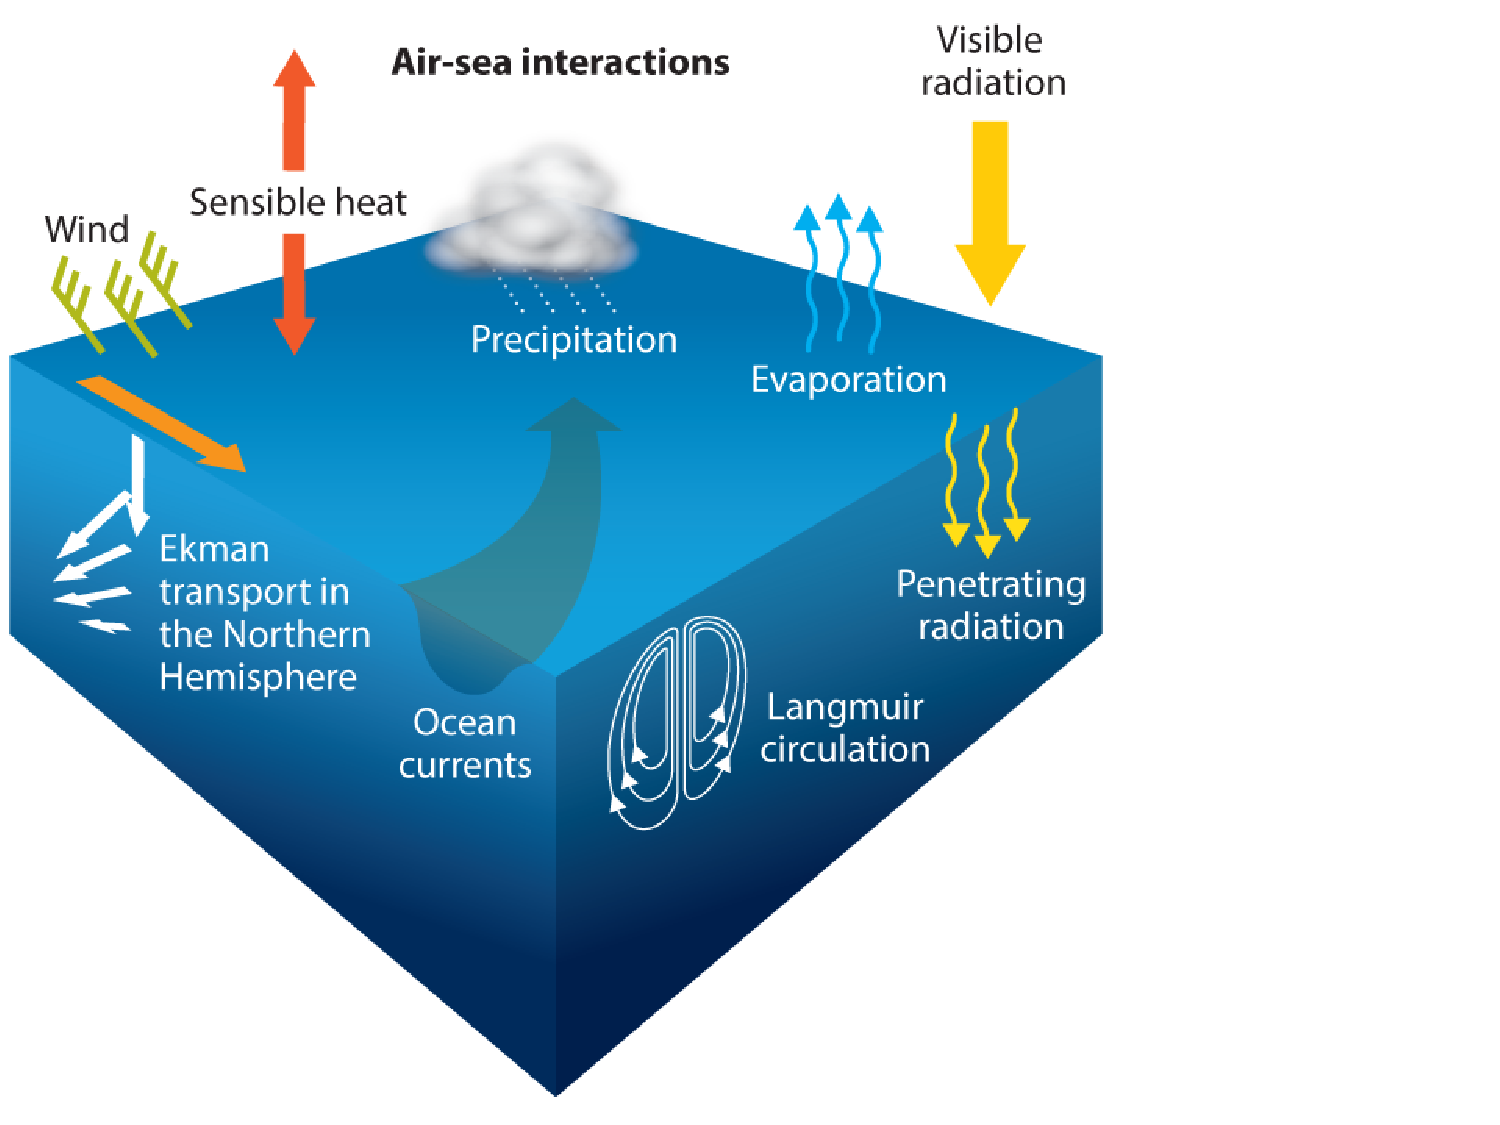
\includegraphics[bb = 0 0 600 550, scale=0.45, clip]{figs/ao_interaction.pdf}
\caption{Schematics of Atmosphere-Ocean interaction(from Encyclopedia of the Environment, https://www.encyclopedie-environnement.org/en/air-en/biosphere-hydrosphere-and-cryosphere-models/)}
\label{fig:ao_interaction}
\end{center}
\end{figure}

Next, a computational aspect of a coupled calculation is described.
Modern high-performance computers operate a plurality of arithmetic units in parallel.
When running a simulation model on a high-performance computer, the model must correspond to the architecture of such a computer.
This correspondence is generally realized through a domain decomposition that divides the model grid.
In addition, in a coupled calculation, a plurality of models are executed in parallel.
Therefore, when exchanging data, it is necessary to conduct a data exchange between appropriate processes in consideration of a domain decomposition.
 \figref{fig:data_exchange_example} shows an example of such a data exchange.
Here, it is assumed that model A has an 8 × 8 grid, and model B has a 12 × 12 grid, and is divided into 4 × 4 and 3 × 3 regions, respectively.
Each region is numbered as shown in the figure.
As indicated by the light green arrow, region 5 of model A exchanges data with regions 0, 1, 3, and 4 of model B.
By contrast, as indicated by the dark green arrows, region 4 of model B exchanges data with regions 6, 7, 10, and 11 of model A.

It is inappropriate to make individual software for conducting such a complex data exchange for each model, and therefore dedicated software for performing a coupled calculation is generally used.
This software is called a coupler or a coupling library.

As mentioned above, there are three main tasks for a coupler:
\begin{enumerate}
\item{Control of data exchange timing}
\item{Grid remapping}
\item{Data exchange between appropriate processes}
\end{enumerate}


\begin{figure}[H]
\begin{center}
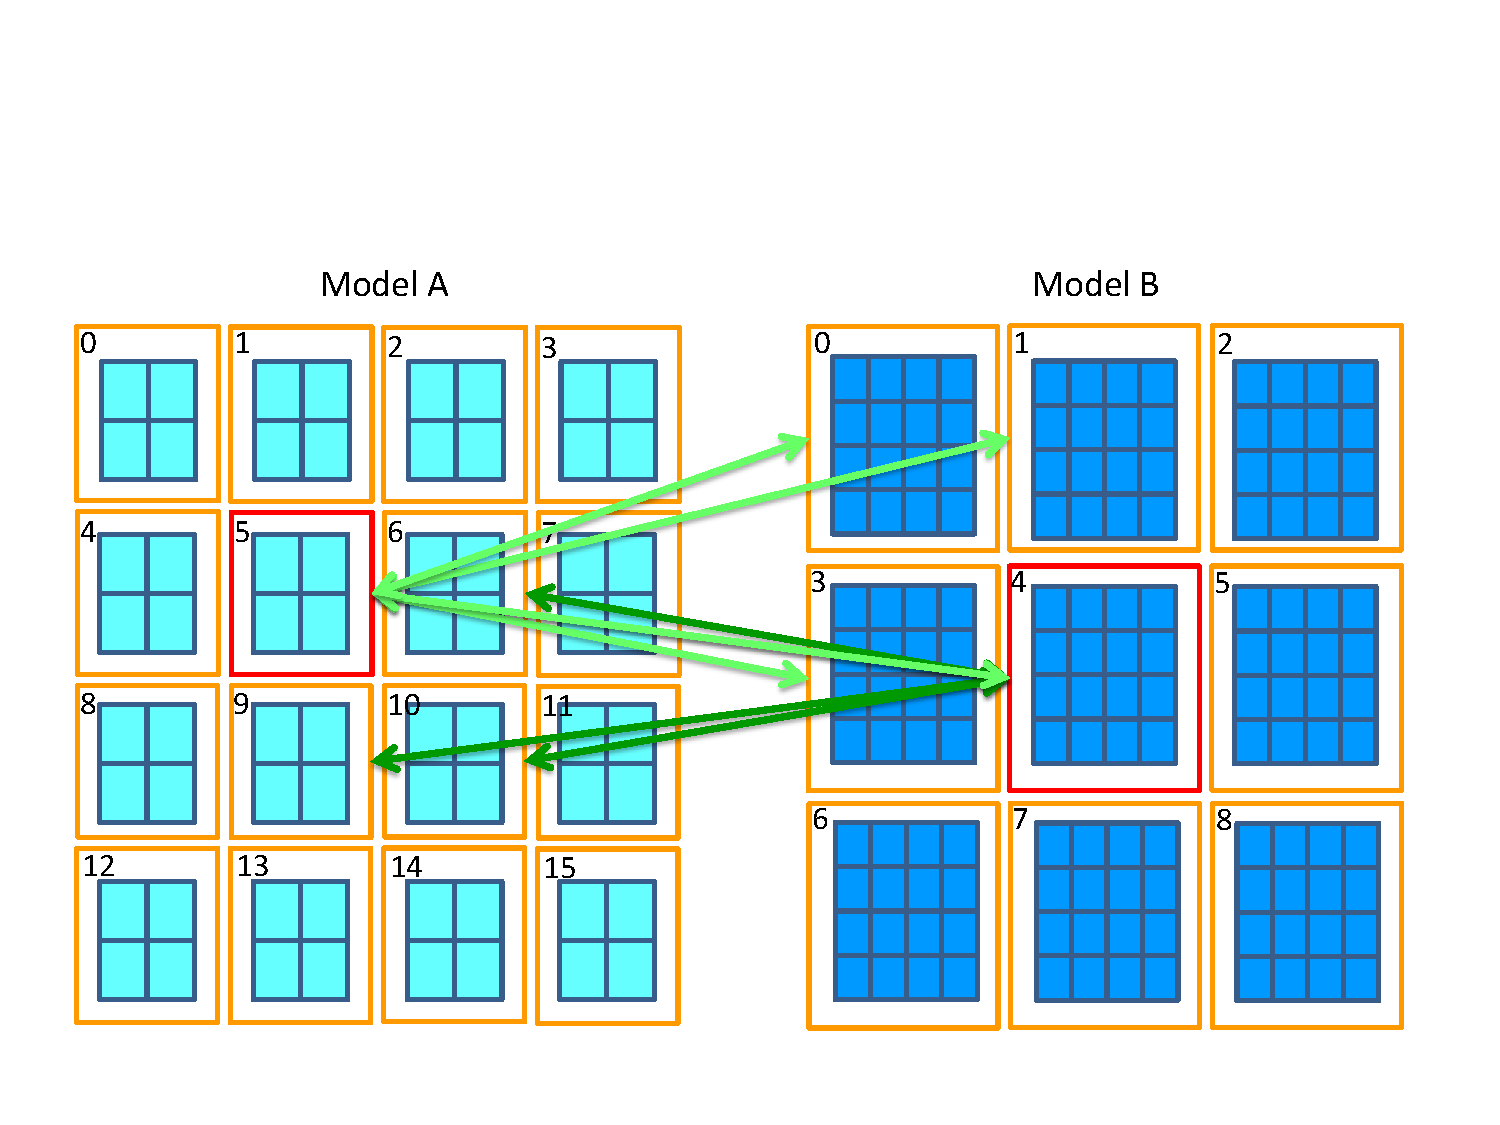
\includegraphics[bb = 0 30 700 450, scale=0.6, clip]{figs/data_exchange_example.pdf}
\caption{Schematic image of data exchange between domain decomposed models.}
\label{fig:data_exchange_example}
\end{center}
\end{figure}

%================================================================================================
%================================================================================================
%================================================================================================

\chapter{Introduction to ILS coupling}
\section{About ILS Coupling System}
An ILS is composed of multiple component models, such as a land surface model, MATSIRO; a river model, CaMa-Flood; and a water resources model, HO8.
To couple these component models, an ILS uses Jcup as a coupling library.
Jcup is a general-purpose coupling library, and there are almost no restrictions on its applicable grid systems and coupling patterns.
However, owing to its high flexibility, its interface is complicated, making it difficult for beginners to use.
Therefore, a wrapper MOJ (MATSIRO Over Jcup) with a more compact interface customized to an ILS was developed.
 MOJ features common to Jcup are summarized as follows.

\begin{itemize}
\item{An arbitrary number of two or more components can be coupled}
\item{Each component can be coupled in series or in parallel}
\item{Each component is parallelized through a domain decomposition}
\item{Any grid system can be applied when it has a uniquely numbered grid}
\item{One component model can have multiple grid systems}
\item{An exchange time interval can be set for all data}
\item{Unlimited number of exchangeable data}
\item{Multiple data can be sent and received together based on the configuration}
\end{itemize}

A user can couple one component model with another by calling the MOJ API subroutines from the model and setting the configuration file.

\section{Coupling Overview}
\subsection{Communicator}
Hereinafter, it is assumed that each component model uses an MPI and is parallelized through a domain decomposition.
A parallel program based on an MPI executes parallel calculations with reference to a communicator.
The default communicator is MPI\_COMM\_WORLD, and there is no problem using this default communicator when running on a single model.
However, when models are coupled using an MOJ, the communicator of each model is generated by the MOJ, and it is therefore necessary to change the communicator to one given by the MOJ.
\figref{fig:moj_mpi_comm} shows a communicator when the component is used alone and a communicator when coupled with an MOJ.
For a single component, MPI\_COMM\_WORLD is used in all component processes.
By contrast, when coupled with an MOJ, MPI\_COMM\_WORLD is defined for all processes of all coupled components, and the communicator of each component is given by the MOJ.
The communicator of each component can be obtained through the MOJ API routine described later.

\begin{figure}[H]
\begin{center}
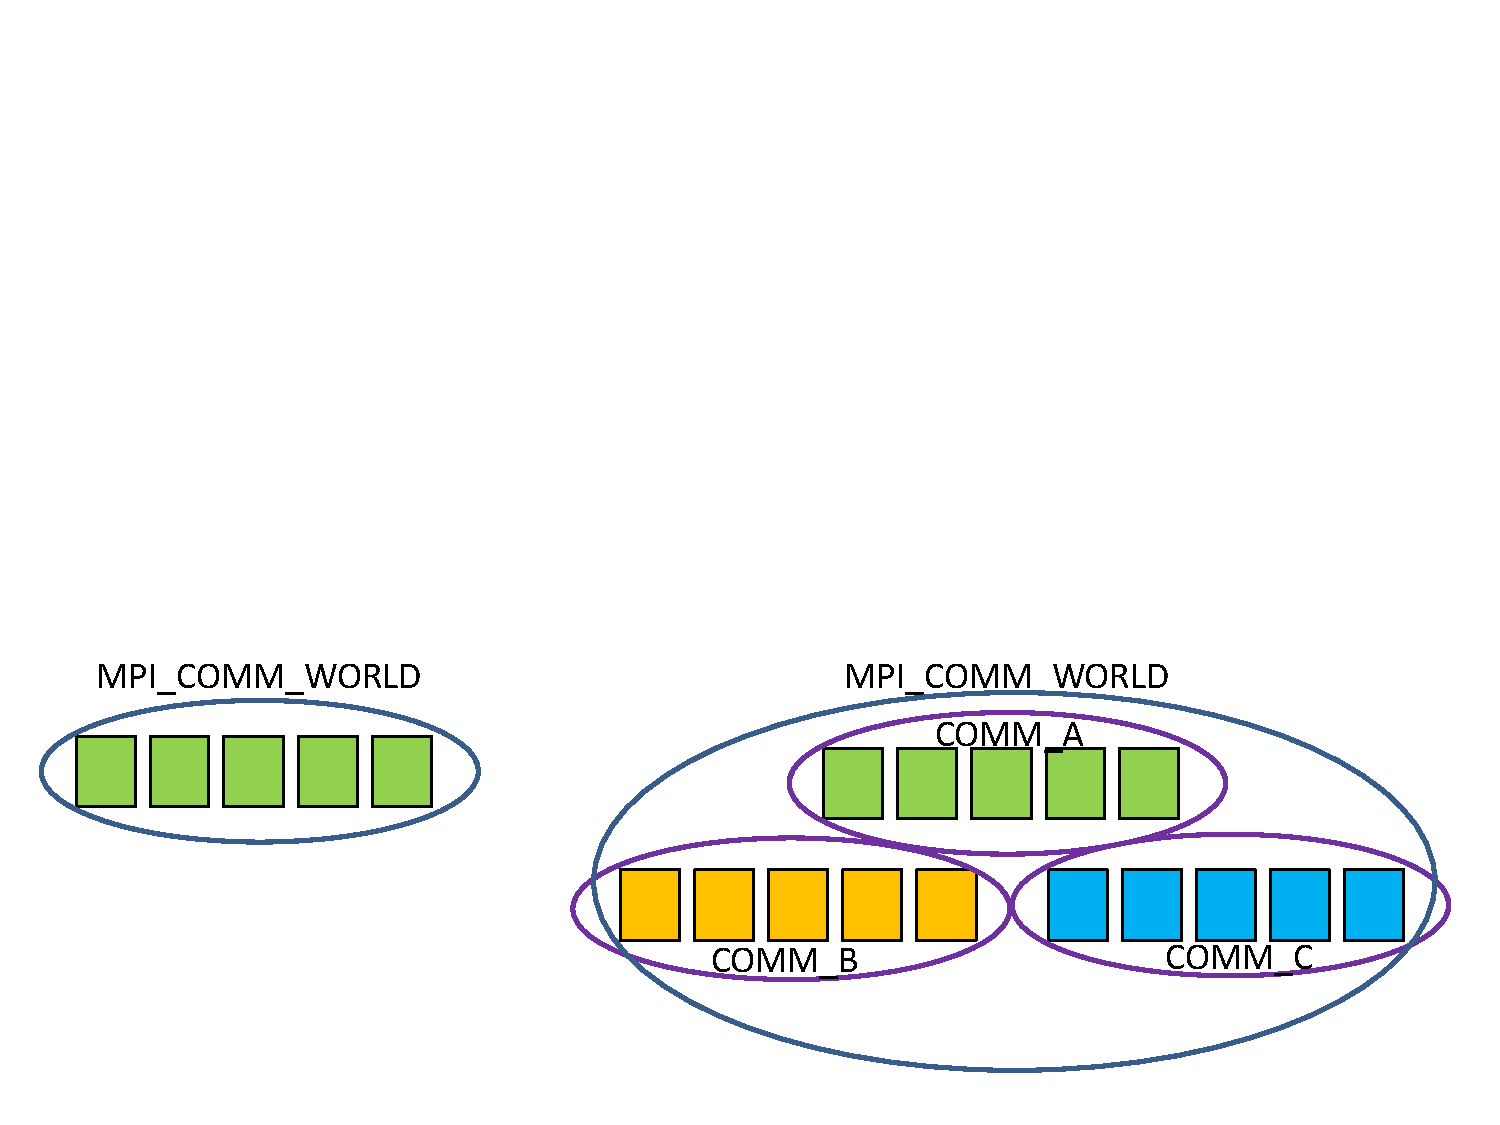
\includegraphics[bb = 0 0 700 300, scale=0.6, clip]{figs/moj_mpi_comm.pdf}
\caption{MPI communicator with components alone and that coupled with an MOJ (left figure; components alone; right figure; components coupled with an MOJ)}
\label{fig:moj_mpi_comm}
\end{center}
\end{figure}

\subsection{Coupling Pattern}
An MOJ can combine two (or more) coupled models in series and in parallel.
Here, serial refers to a case in which two components pass data during the same time step, and parallel refers to a case in which two components pass data of a previous time step to each other.
A schematic diagram of both patterns is shown in \figref{fig:coupling_pattern}.
The left figure is a serial coupling example, in which the calculation result of model A is passed to model B during the same time step, and the calculation of model B is conducted.
In serial coupling, each model component waits for the end of the calculation of the other component, and thus the overall execution time is substantially equal to the sum of the execution times of the two components.
The right figure shows an example of a parallel coupling, where the model component sends the calculation result to the other side component at each time step, and receives the data of the other side component at the next time step.
In this case, the overall execution time is approximately equal to the time of the component with the longest execution time.
The gray squares before $ T_0 $ indicate the initial value exchange.

\begin{figure}[H]
\begin{center}
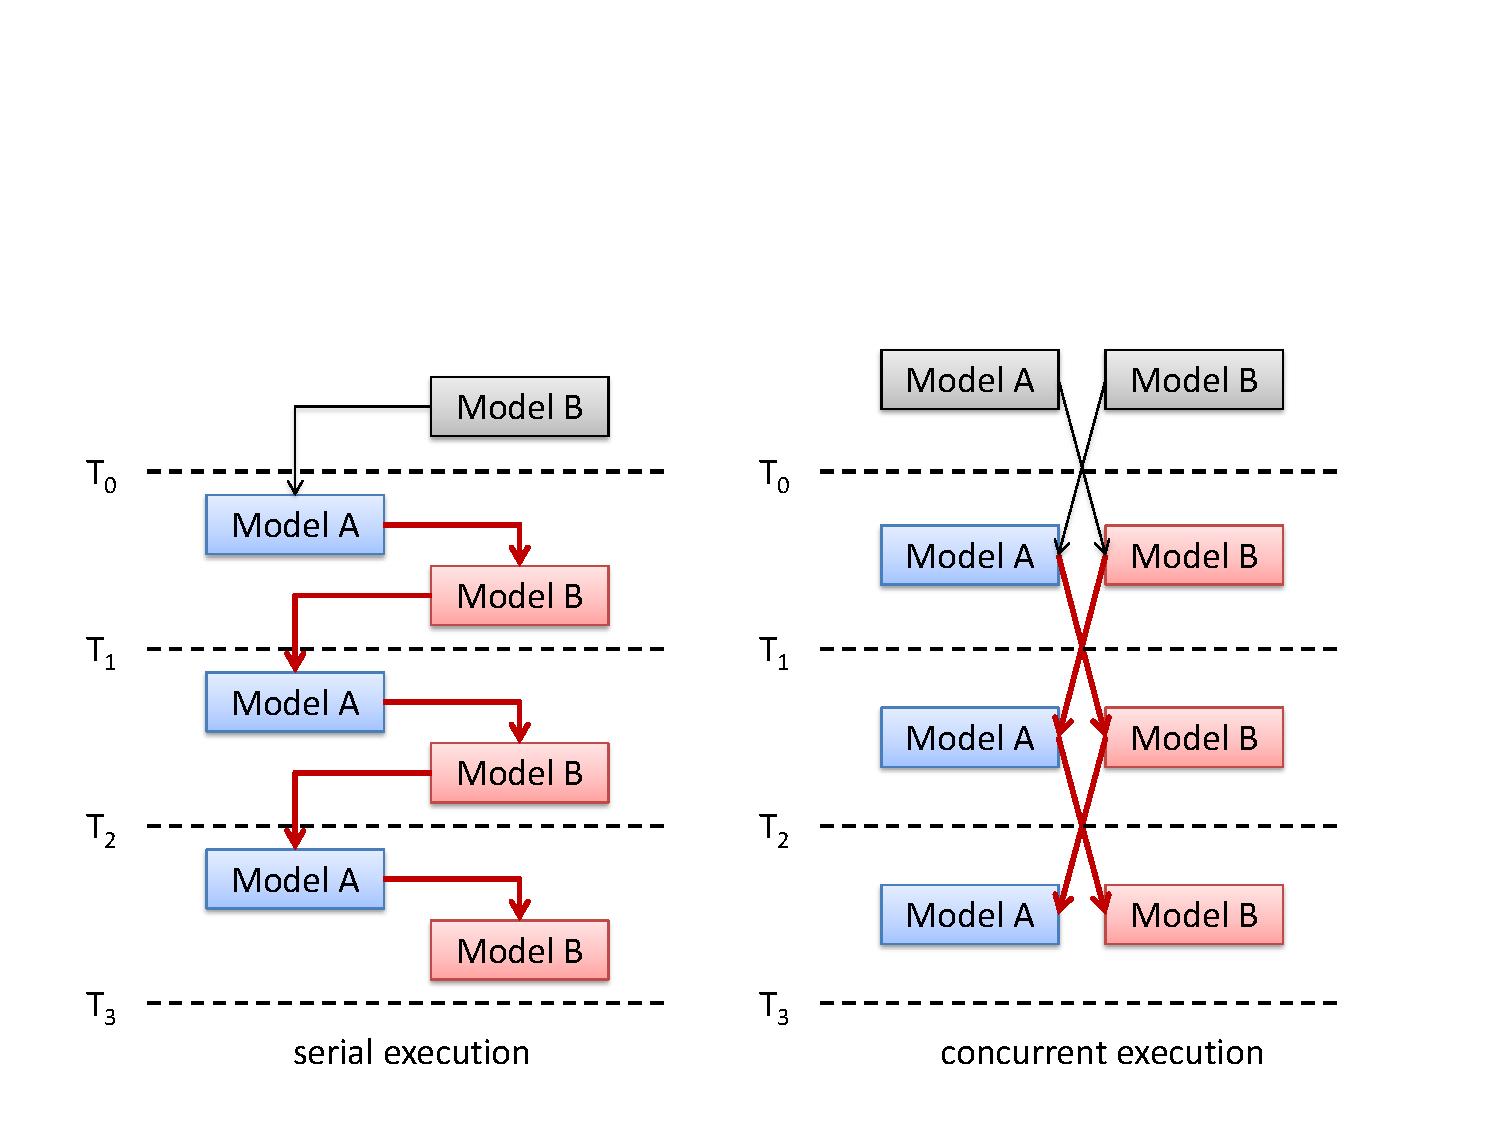
\includegraphics[bb = 0 0 700 400, scale=0.6, clip]{figs/coupling_pattern.pdf}
\caption{Coupling pattern(left:serial coupling,right:parallel coupling)}
\label{fig:coupling_pattern}
\end{center}
\end{figure}

\subsection{Data Exchange}
The data exchange time interval can be set for each data.
In the example shown in \figref{fig:data_exchange_pattern}, model B exchanges data with model C every four steps, and model A every five steps.
At the time of a data exchange, each model requires that the model time coincide with the data exchange time.
Time steps other than the data exchange time do not need to be constant.

\begin{figure}[H]
\begin{center}
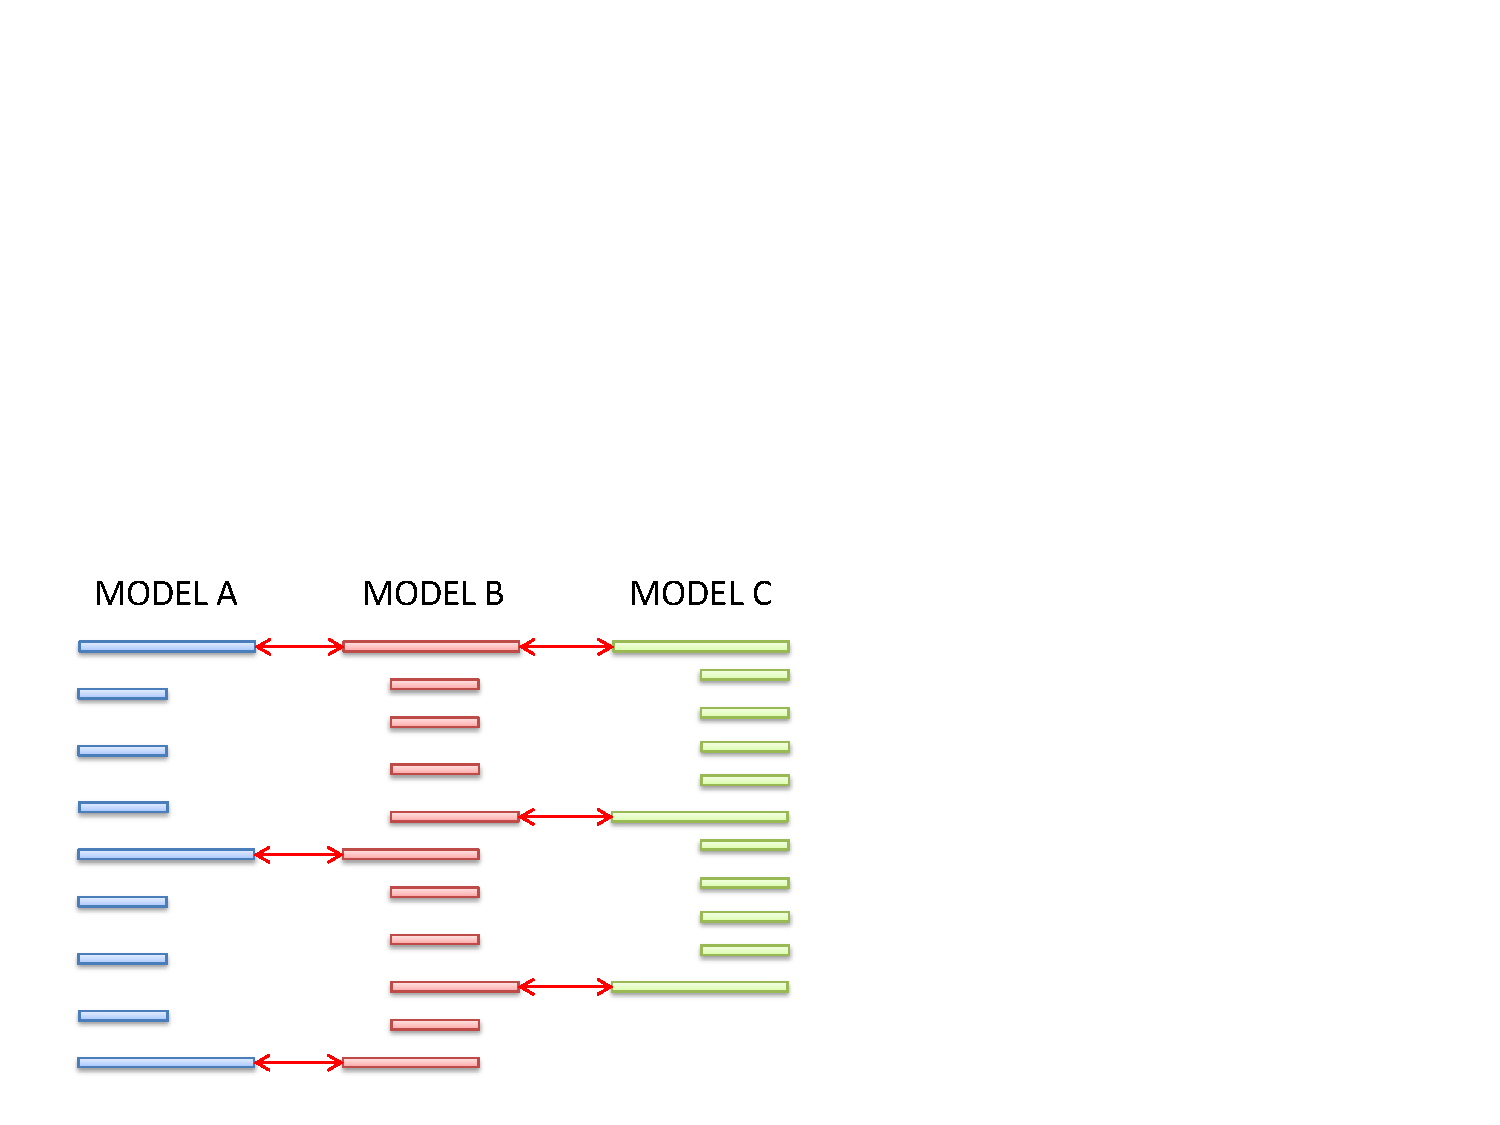
\includegraphics[bb = 0 0 500 300, scale=0.6, clip]{figs/data_exchange_pattern.pdf}
\caption{Data exchange pattern}
\label{fig:data_exchange_pattern}
\end{center}
\end{figure}



%================================================================================================
%================================================================================================
%================================================================================================
\chapter{Preparation}
\section{Grid index table}
Which region (MPI process) of the target component to which all grid point data are exchanged is determined by the grid point index assigned to each area of the component model and the mapping table described in the next section.

The grid point index of the grid assigned to each region is given to the coupler by the MOJ API subroutine moj\_def\_grid.
The index must be made up of natural numbers. In addition, it does not need to be continuous, and a discrete number can be applied.

However, the numbers need to be unique among the grid points of all regions.
Because the coupler does not check for duplicate numbers, an operation in the presence of duplicate grid points cannot be predicted.
One component can have a plurality of grids, and the number of grid points and the grid point index of each grid can be set independently.


\section{Mapping table}
An MOJ does not depend on the grid structure and can flexibly couple the models whose grid does not change over time.
However, for this purpose, it is necessary to obtain the correspondence between grid indexes among the models and the interpolation coefficients in advance.
For example, as shown in \figref{fig:interpolation_image}, the value of grid point R(p) of the receiving model is calculated from grid points $S(i)-S(i+4)$ and coefficient $Cs(i)-Cs(i+4)$, as shown the equation below:

\begin{equation}
R(p) = \sum_{n=0}^{4} Cs(i+n)*S(i+n)
\end{equation}

The mapping table for $R(p)$ can be expressed as \lstref{list:mapping_table_sample}. 
For the vector quantity, a coefficient expressing rotation is further added. 
These values are given as arguments of the MOJ API subroutine moj\_set\_interpolation\_table to be described later.


\begin{figure}[H]
\begin{center}
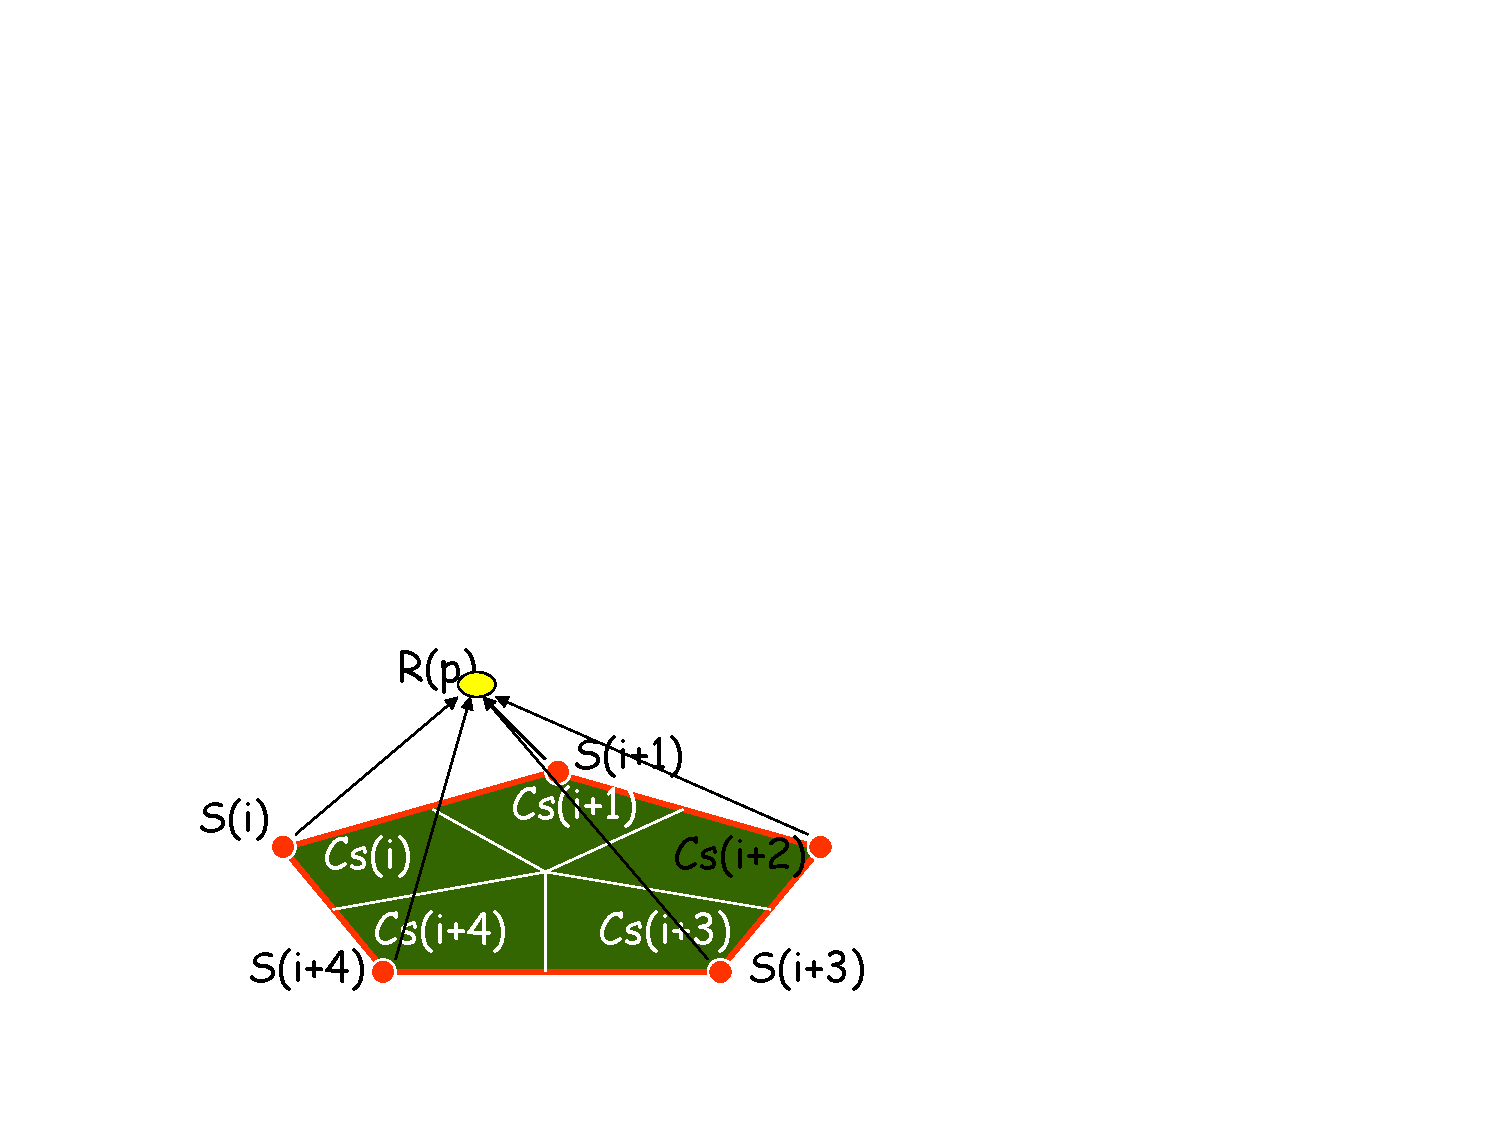
\includegraphics[bb = 0 0 500 250, scale=0.6, clip]{figs/interpolation_image.pdf}
\caption{Grid points and coefficients on interpolation calculation}
\label{fig:interpolation_image}
\end{center}
\end{figure}

\begin{lstlisting}[caption=Example of mapping table, label=list:mapping_table_sample]
 R(p), S(i), Cs(i)
 R(p), S(i+1), Cs(i+1)
 R(p), S(i+2), Cs(i+2)
 R(p), S(i+3), Cs(i+3)
 R(p), S(i+4), Cs(i+4)
\end{lstlisting}

\section{Configuration file}
To define the operation of an MOJ, it is necessary to create a configuration file in advance. 
The name of the configuration file is given by the MOJ API subroutine moj\_init. 
What users need to set in the configuration file are the coupler\_config session, which specifies the operation of the coupler, and the nam\_moj session, which defines the exchange data.
The elements, descriptions, and possible values for each session are summarized in \tabref{table:coupler_config} and \tabref{table:nam_moj_var}.

The session coupler\_config consists of two elements, log\_level and debug\_mode. 
Of these, log\_level sets the detailedness (amount) of the log output. Possible values include "SILENT," "WISPER," and "LOUD." 
The latter value outputs a more detailed log. 
Debug\_mode is a flag indicating whether to output a log. 
If debug\_mode = .false., a log is not output regardless of the log\_level setting.
Note that log\_level = "LAUD" outputs a large number of logs, and thus care must be taken when performing long-term integration.

The session nam\_moj describes the sending/receiving components, the grid, and the data group exchanged between these components.
A plurality of data can be set for a pair of components and a grid, and all data are interpreted as corresponding to the component and the grid described immediately before.
Settings that can be omitted are shown in italics in the table.

Var\_put and var\_get are exchange data names, and var\_put\_vec and var\_get\_vec are exchange vector data names. 
Either a scalar data name or a vector data name must be specified.
Mapping\_tag is a tag for specifying a mapping table.
Time\_intpl\_tag is a data identification tag for time interpolation, and data with the same numbered tag are passed to the time interpolation subroutine of the IO component.
This tag is valid only when coupling IO components.
Grid\_intpl\_tag is a data identification tag for spatial interpolation, and data with the same number are exchanged as a set of data and passed to the spatial interpolation subroutine.
Intvl sets the data exchange interval in seconds.
Lag sets the coupling pattern. When two components are coupled in parallel, a value of -1 is given to both the sending and receiving data, and when they are coupled in series, a value of 1 is given to the preceding component and a value of -1 is given to the succeeding component. In addition, 0 indicates a special setting, and is set only when the initial data are acquired from the IO component using the API subroutine moj\_get\_initial\_data described later.
Layer is an integer indicating the number of vertical layers of data.
Flag is a flag indicating whether to calculate the time average internally, and specifies "SNP" or "AVR."
Factor is a real constant that is multiplied with the data at the spatial interpolation.
Is\_ok is a flag indicating whether a data exchange is actually conducted.
If is\_ok = 1, the data are exchanged, and if the value is 0, the data are not exchanged.
A sample of the configuration file is shown in \lstref{list:moj_namelist_sample}.

\begin{table}[H]
\begin{center}
\caption{Elements of couple\_config session of configuration file}
{\small
\label{table:coupler_config}
\begin{tabular}{lll}
\hline\hline
 element name & description & possible values \\
\hline
 log\_level & log output level & one of "SILENT," "WISPER," "LOUD"\\
 debug\_mode & Flag to output log or not & .true. or .false.\\
\hline\hline
\end{tabular}
}
\end{center}
\end{table}

\begin{table}[H]
\begin{center}
\caption{Example of nam\_moj section (component and grid setting)}
{\small
\label{table:nam_moj_comp}
\begin{tabular}{lll}
\hline\hline
 element name & description & possible value \\
\hline
 comp\_put & sending component name & string of the component name\\
 comp\_get & receiving component name & string of the component name\\
 grid\_put & grid name of the sending component & string of the grid name\\
 grid\_get & grid name of the receiving component & string of the grid name\\
\hline\hline
\end{tabular}
}
\end{center}
\end{table}

\begin{table}[H]
\begin{center}
\caption{Example of nam\_moj section (exchange data setting)}
{\small
\label{table:nam_moj_var}
\begin{tabular}{lll}
\hline\hline
 element name & description & possible value \\
\hline
 var\_put & send data name & string of the name\\
 var\_get & receive data name & string of the name\\
 var\_put\_vec & send vector data name & string of the name\\
 var\_get\_vec & receive vector data name & string of the data name\\
 {\it mapping\_tag} & mapping table tag & integer for specifying the mapping table\\
 {\it time\_intpl\_tag} & time interpolation tag & integer for identifying the data\\
 {\it grid\_intpl\_tag} & spacial interpolation tag & integer for identifying the data\\
 intvl & data exchange interval & integer in second\\
 lag   & coupling pattern & -1 or 0 or 1\\
 {\it layer} & number of vertical layer & integer for vertical layer (default 1)\\
 flag  & time averaging flag & "SNP" or "AVR"\\
 {\it factor} & value multiplied to the data & real(kind=8) (default 1)\\
 {\it is\_OK} & flag to exchange the data or not & 1 or 0 (default 1)\\
\hline\hline
\end{tabular}
}
\end{center}
\end{table}

\begin{lstlisting}[caption=Example of MOJ configuration, label=list:moj_namelist_sample]
&coupler_config
  log_level = "LOUD"
  debug_mode  = .true.
&end 


&nam_moj  comp_put = "MATIO",   comp_get = "MATSIRO",
          grid_put ='io_grid', grid_get ='matsiro_grid', /
&nam_moj  var_put = 'SWdown'    ,  var_get ='SWdown'    , time_intpl_tag = 1, grid_intpl_tag = 1, intvl=3600 ,  lag=-1, flag='SNP' /
&nam_moj  var_put = 'LWdown'    ,  var_get ='LWdown'    , time_intpl_tag = 2, grid_intpl_tag = 1, intvl=3600 ,  lag=-1, flag='SNP' /
&nam_moj  var_put = 'Rainf'     ,  var_get ='Rainf'     , time_intpl_tag = 2, grid_intpl_tag = 1, intvl=3600 ,  lag=-1, flag='SNP' /
\end{lstlisting}


%================================================================================================
%================================================================================================
%================================================================================================
\chapter{How to use the API subroutines}
\section{Overview of their usage}
To use the MOJ component model, make the API module moj\_api available in the use statement. 
A typical usage of the MOJ API routine is as follows: \figref{fig:moj_usage_sample}. 
First, initialize the MOJ with moj\_init, and make various settings related to the MPI. 
Next, various information of the MPI set by the MOJ is acquired by moj\_get\_comm\_local and moj\_get\_irank\_local. 
Set the grid point index of each area of the component with moj\_def\_grid, and notify the MOJ of the end of the setting with moj\_end\_grid\_def. 
Set the mapping table with moj\_set\_interpolation\_table and give the initial time to the MOJ with moj\_init\_time. 
Provide the initial value with moj\_put\_data if necessary. 
Finally, tell the MOJ about the end of the join with moj\_finalize.


\begin{figure}[H]
\begin{center}
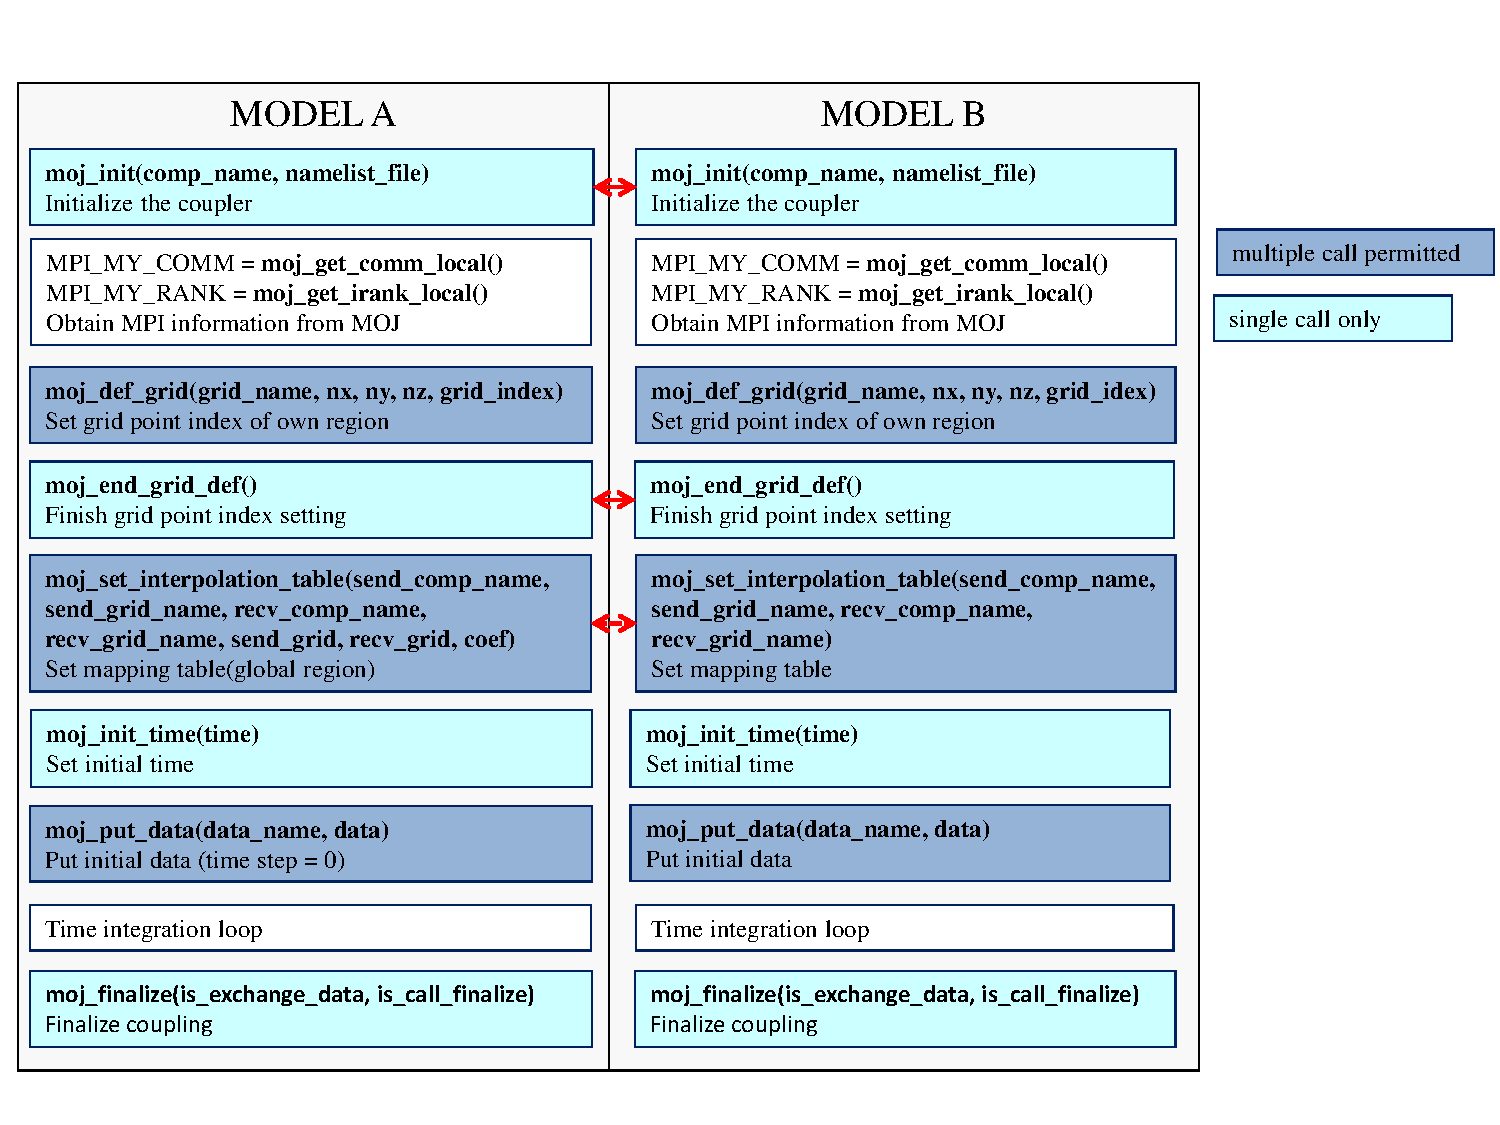
\includegraphics[bb = 0 25 750 520, scale=0.59, clip]{figs/moj_usage_sample.pdf}
\caption{Typical usage of MOJ API routines during the initialization phase}
\label{fig:moj_usage_sample}
\end{center}
\end{figure}

The call and internal operation of the MOJ API in the time integration loop are as shown in \figref{fig:moj_time_integ}.
There are three API routines used in the time integration loop: moj\_set\_time, moj\_get\_data, moj \_put\_data.
Call moj\_set\_time near the beginning of the time integration loop and give the current time and $\Delta{T}$ to the MOJ.
Data exchange and interpolation calculations are conducted inside this routine.
Obtain the data of the target component with moj\_get\_data, execute the calculation, and pass the result to the MOJ with moj\_put\_data.
It should be noted that these API routines must be called for every time step.

\begin{figure}[H]
\begin{center}
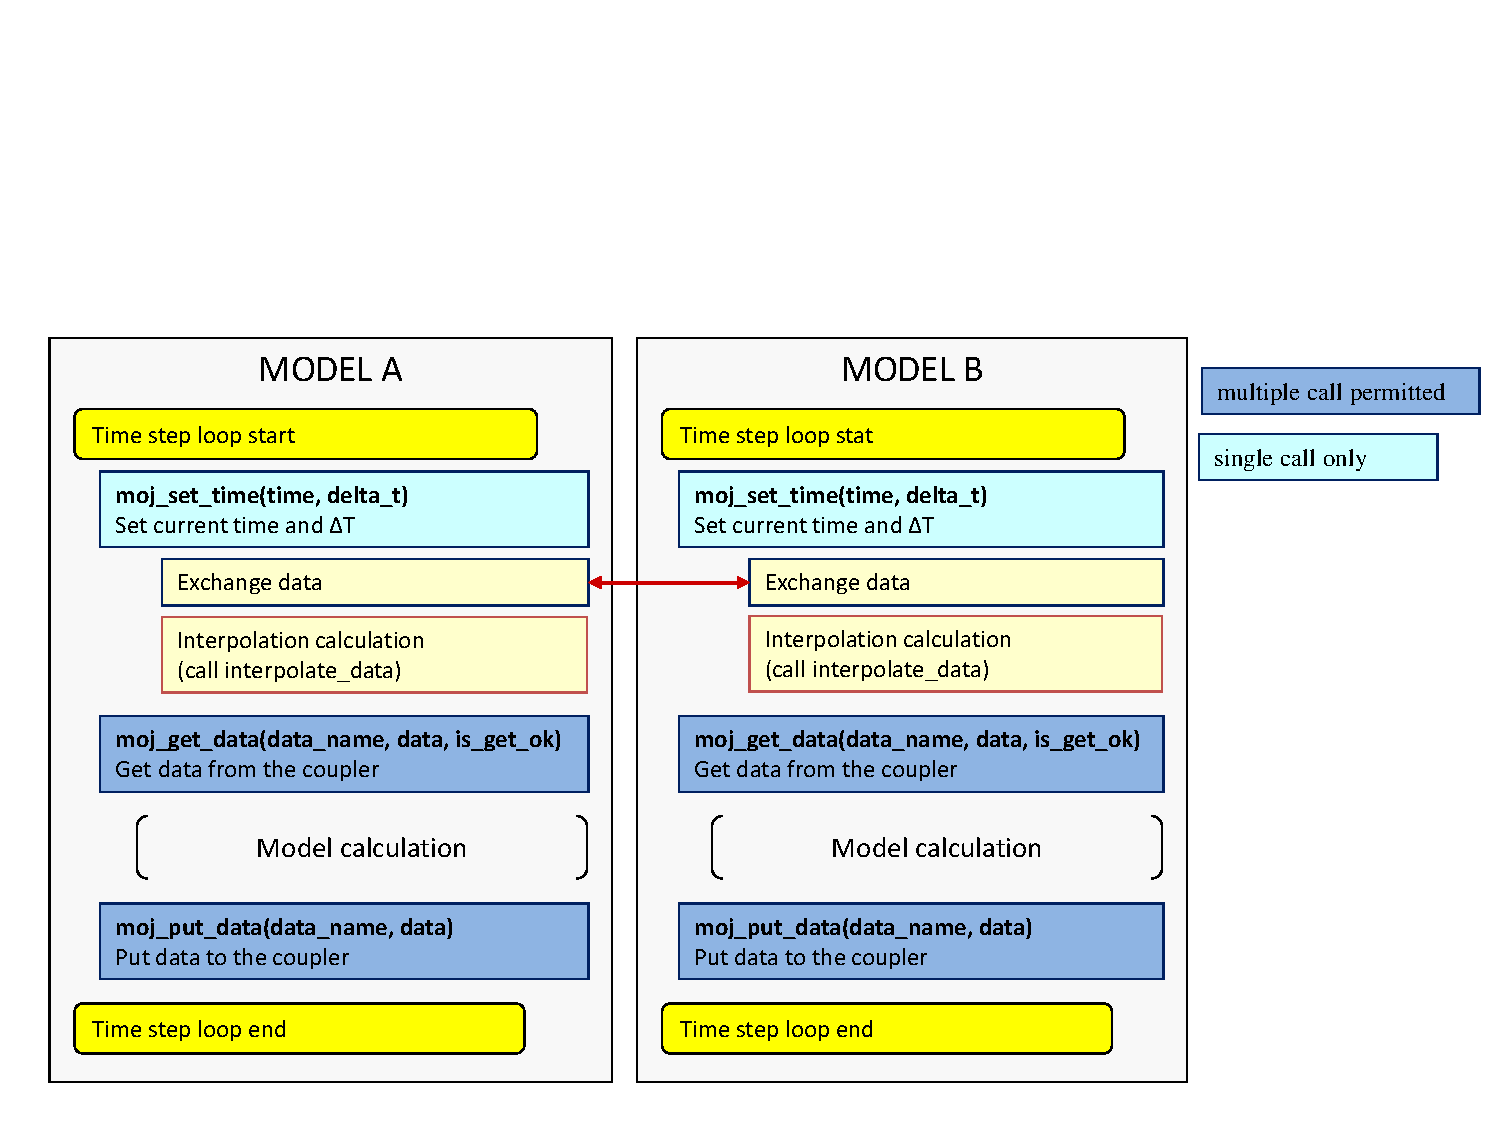
\includegraphics[bb = 0 0 750 400, scale=0.6, clip]{figs/moj_time_integ.pdf}
\caption{Typical usage of MOJ API routines in the time integration loop}
\label{fig:moj_time_integ}
\end{center}
\end{figure}

\section{Initialize MOJ}
First, initialize the MOJ with moj\_init. 
The arguments are the name of the component and the name of the configuration file. 
If the MPI initialization subroutine MPI\_Init is not called in the model component, it is called inside this routine. 
Note that calling MPI\_Init on the model component after calling moj\_init will result in a double call error.

\section{Get MPI information}
As shown by \figref{fig:moj_mpi_comm}, the MPI communicator of each component when coupled by the MOJ is generated inside the MOJ. Therefore, the communicator used when a component calls an MPI routine must be the one generated by the MOJ. 
The communicator generated by the MOJ can be obtained using the API function moj\_get\_comm\_local. 
In addition, the process number inside the component can be obtained from the MOJ API routine.

\section{Set grid index}
Set the grid point number with moj\_def\_grid. 
The arguments are a grid name, a grid size $(nx, ny, nz)$, and a one-dimensional array grid\_index(:) of the grid point indexes. 
What should be noted here is whether to include the vertical dimension in the array of the grid point indexes to be given. 
For example, in the case of atmosphere-ocean coupling, the exchange data are two-dimensional horizontally, and even if a third dimension exists, in numerous cases, it is not a physical vertical layer but a quantity such as a category. 
Further, even when exchanging data such as atmosphere and chemistry coupling in a physical three-dimensional space, the grid differs only in the horizontal plane, and vertical interpolation may not be necessary in certain cases. 
When the mapping table is expressed only in the horizontal plane as in these examples, even if the data to be exchanged have a vertical layer, the grid index setting is $ nz = 1 $, and the size of the grid\_index is $nx *ny$.
The above is summarized as follows.

\begin{itemize}
\item{When the exchange data are horizontal 2D data or the interpolation calculation is horizontally 2D only}

nz = 1, and grid\_index is given as an array of size $nx * ny$.

\item{Interpolation calculation in 3D space including vertical}

grid\_index is given as an array of size $nx * ny * nz$.

\end{itemize}

When exchanging 3D data including a vertical layer in the former case, the number of vertical layers is given to the layer by setting individual data in the setting file.


\section{Set mapping table}
The mapping table setting subroutine moj\_set\_interpolation\_table must be called by both the sending component and the receiving component. 
Because a data exchange is conducted inside this subroutine, the calling location must correspond in the sending and receiving components. 
Arguments after the grid point index are optional arguments and are given by the receiving component. 
Further, when the data to be exchanged are only of a scalar amount or there is no rotation of the grid, it is not necessary to provide two arguments of coef\_sin and coef\_cos. 
The above results are shown in \tabref{table:interpolation_table_arguments}.

\begin{table}[H]
\begin{center}
\caption{Arguments of moj\_set\_interpolation\_table}
{\small
\label{table:interpolation_table_arguments}
\begin{tabular}{|ll|l|}
\hline
 Arguments & meaning & Criteria to give \\
\hline
 send\_comp\_name & send component name &\\
 send\_grid\_name & send grid name & give both\\
 recv\_comp\_name & receive component name & component\\
 recv\_grid\_name & receive grid name & \\
\hline
 send\_index & send grid index & give on the \\
 recv\_index & receive grid index & receive component \\
 coef        & interpolation coefficient & \\
\hline
 coef\_sin   & rotation coefficient & give on the receive component\\
 coef\_cos   & rotation coefficient & and rotation is necessary\\
\hline
\end{tabular}
}
\end{center}
\end{table}


\section{Set initial time}
Give the initial time with moj\_set\_init\_time. 
The argument is an integer array of size 6, representing the year, month, day, hour, minute, and second.

\section{Initial value Put}
Before entering the time integration loop, the sending side must put the data received in the first step. The API subroutine is moj\_put\_data or moj\_put\_data\_vec, and the arguments are the data name and data (one variable for the scalar data and two variables for the vector data).

\section{Time integration}
\subsection{Setting of current time and $\Delta{T}$}
Call the API routine moj\_set\_time in the time integration loop and give the current time and $\Delta{T}$. The arguments are an integer array of size 6 representing the year, month, day, hour, minute, and second, and an integer representing $\Delta{T}$. 
Note that (currently) the unit of $\Delta{T}$ is only in seconds.
Because processing inside the coupler, such as a data exchange determination, uses the integrated value of $\Delta{T}$, moj\_set\_time must be called at every step.

\subsection{Obtaining the data}
To obtain the target data, call moj\_get\_data or moj\_get\_data\_vec. 
The argument data\_name is the data name, and data, or data1, data2, is the receiving data array.
The optional argument data\_scalar is a scalar quantity received at the same time as these data, and the optional argument data\_scalar must also be given in moj\_put\_data of the corresponding target component.
The optional argument is\_get\_OK is a logical type argument that returns whether the step is a data receiving step.

\subsection{Putting the data}
To send data, moj\_put\_data or moj\_put\_data\_vec is called, which is the same as the initial value, Put. 
The argument data\_name is the data name, and data, or data1 and data2, are sending data arrays. 
The optional argument data\_scalar is the scalar quantity to be sent at the same time as these data. 
If the step is not a sending step, the processing is appropriately conducted (sending is skipped) inside the coupler, and thus it is not necessary for the user to make a call determination according to the step.

\section{Ending process}
Finally, moj\_finalize is called at the end of the coupling. 
The argument is\_exchange\_data is a flag for sending/receiving the last step data inside moj\_finalize when the last step data are not sent/received owing to the time integration step algorithm. Here,
"is\_call\_finalize" is a flag indicating whether to call the MPI termination routine MPI\_finalize internally.

\section{Other main routines}
\subsection{Get initial value}
The subroutine moj\_get\_initial\_data is used to obtain the initial value from the IO component. 
The arguments are a data name and an array to obtain the data. 
This subroutine must be called before the time integration. 
In addition, it is necessary to set the reading of the initial value in the configuration file used by the IO component.

\subsection{Get MPI information}
In addition to the communicator acquisition function moj\_get\_comm\_local, moj\_get\_irank\_local, which returns the rank of its own component, and moj\_get\_numpe\_local, which returns the number of ranks, are provided. 
A subroutine moj\_get\_mpi\_parameter for obtaining MPI information at a particular time is also provided.

\subsection{Data exchange}
Moj\_send\_value and moj\_recv\_value are provided as subroutines for sending data to and receiving data from the target component. 
The argument is a character string comp\_name representing the name of the target component and a character string, or an integer, an integer array, a real number, or a real number array, representing a data exchange.

\subsection{Calendar operation routine}
A subroutine group for adding/subtracting the date, month, day, hour, minute, and second according to the type of calendar and calculating the difference between two times is provided. 
See the reference for details regarding this content.

\subsection{Setting information acquisition routine}
Although not required for normal use of the MOJ, there are routines that return the settings in the configuration file for special purposes. 
See the references for details on the individual routines.

\subsection{Log output routine}
Here, moj\_put\_log outputs a Jcup format log to a Jcup log file. The argument sub\_name is the name of the subroutine, and log\_str is the character string of the log.

\subsection{Execution information acquisition routine}
Here, moj\_is\_coupled is a function that returns whether the component specified by the argument comp\_name is currently running (coupled).


%================================================================================================
\chapter{References}
\section{APIs of MOJ}
\subsection{Public constants}
The constants published by the MOJ are shown in \tabref{table:moj_constant}. 
These are all constants for specifying the type of calendar to be used, and are used as arguments of the API subroutine moj\_init\_calendar described later. 
CALENDAR\_NORLAM indicates that a normal Gregorian calendar is used, CALENDAR\_NOLEAPYEAR uses a calendar fixed at 365 days a year without leap years, and CALENDAR\_30360 indicates that a calendar is fixed at 360 days a year, and 30 days a month.

\begin{table}[H]
\begin{center}
\caption{Public constants of MOJ}
{\small
\label{table:moj_constant}
\begin{tabular}{ll}
\hline\hline
 name & description \\
\hline
 CALENDAR\_NORMAL & Use regular Gregorian calendar\\
 CALENDAR\_NOLEAPYEAR & Use a fixed calendar of 365 days a year without considering leap years\\
 CALENDAR\_30360 & Use a fixed calendar of 30 days a month, 360 days a year\\
\hline\hline
\end{tabular}
}
\end{center}
\end{table}

\subsection{Initialization APIs}
The MOJ API subroutine group related to initialization is shown in \tabref{table:moj_api_initialize}.
Subroutine moj\_init initializes the MOJ. 
The argument is a character string representing the component name and the configuration file name. This subroutine is called only once.
The subroutine moj\_def\_grid sets the grid used by each component. 
The argument grid\_name represents the name of the grid. 
In addition, nx, ny, and nz represent the size of the grid assigned to the area. 
In a model such as CaMa, which expresses grid points in one dimension, nx is the given grid size, and ny and nz may be set to 1. 
grid\_index is an integer array indicating the grid point index of the grid in charge of its own area. 
This subroutine can be called multiple times depending on the number of grid systems coupled.
The subroutine moj\_end\_grid\_def declares the end of the grid definition.

The subroutine moj\_set\_interpolation\_table sets the grid point correspondence and interpolation coefficients used in an interpolation calculation. 
The arguments send\_comp\_name, send\_grid\_name, recv\_comp\_name, and recv\_grid\_name represent a send component name, a send grid name, a receive component name, and a receive grid name, respectively. 
In addition, “send\_index” and “recv\_index” are the grid point indexes on the sending and receiving sides in the interpolation calculation. 
The correspondence for all regions is given, and the size of the two arrays must match. 
Note that this argument may be given by the route processor of the receiving component. 
Here, "coef" is an array corresponding to the interpolation coefficient $C$ when calculating $R = R + S * C$, and
"coef\_sin" and "coef\_cos" are rotation coefficients when the rotating vector quantities are $U = u*coef\_cos*u-coef\_sin*v$ and $V = coef\_sin*u + coef\_cos*v$.
The subroutine moj\_init\_time sets the initial time of the calculation. 
The argument time\_array(:) is an integer of size 6 representing the year, month, day, hour, minute, and second.

Note that these subroutines must be called in the order shown in the table.

\begin{table}[H]
\begin{center}
\caption{Initialization API of MOJ}
{\small
\label{table:moj_api_initialize}
\begin{tabular}{llll}
\hline\hline
routine name & type of argument & argument & description \\
\hline
 moj\_init &  \multicolumn{3}{l}{initialize MOJ}\\
           &  character(len=*), intent(IN) &  comp\_name & component name\\
           &  character(len=*), intent(IN) &  namelist\_file & configuration file name\\
\hline
 moj\_def\_grid & \multicolumn{3}{l}{set grid index} \\ 
                & character(len=*), intent(IN) & grid\_name & grid name\\
                & integer, intent(IN) & nx & number of local grid points\\ 
                &                     &    & in i-direction\\
                & integer, intent(IN) & ny & number of local grid points\\
                &                     &    & in j-direction\\
                & integer, intent(IN) & nz & number of local grid points\\
                &                     &    & in k-direction\\
                & integer, intent(IN) & grid\_index(:) & grid point index \\
                &                     &    & of local grid\\
\hline
 moj\_end\_grid\_def &  \multicolumn{3}{l}{end grid setting}\\
                & no argument & & \\
\hline
 moj\_set\_ & \multicolumn{3}{l}{set mapping table} \\ 
 interpolation\_table & character(len=*), intent(IN) & send\_comp\_name & send component name\\
                & character(len=*), intent(IN) & send\_grid\_name & send grid name\\
                & character(len=*), intent(IN) & recv\_comp\_name & receive component name\\
                & character(len=*), intent(IN) & recv\_grid\_name & receive grid name\\
                & integer, optional, intent(IN) & send\_index(:) & grid index of \\
                &                               &                & send component\\
                & integer, optional, intent(IN) & recv\_index(:) & grid index of \\
                &                               &                & receive component\\
                & real(kind=8), optional, intent(IN) & coef(:) & interpolation coefficient\\
                & real(kind=8), optional, intent(IN) & coef\_sin(:) & rotation coefficient(sin) \\
                & real(kind=8), optional, intent(IN) & coef\_cos(:) & rotation coefficient(cos) \\
\hline
 moj\_init\_time &  \multicolumn{3}{l}{set initial time}\\
                & integer, intent(IN) & time\_array(:) & integar array \\
                &                     &                & yy/mo/dd/hh/mm/ss\\
\hline
 moj\_get\_initial\_data & \multicolumn{3}{l}{get initial data} \\ 
                & character(len=*), intent(IN) & data\_name & data name\\
                & real(kind=8), intent(INOUT) & data(:),data(:,:),data(:,:,:) & receive data\\
                & logical, intent(OUT)        & is\_get\_ok & receive data flag\\
\hline\hline
\end{tabular}
}
\end{center}
\end{table}


\subsection{APIs in the time integration loop}
API subroutines for exchanging data in the time integration loop are shown in \tabref{table:moj_api_integration}.
The subroutine moj\_set\_time is given an integer array of size 6 representing the current time and an integer representing $\Delta{T}$. 
This subroutine is to be called at the beginning of the time integration loop, and data exchanges are executed within this subroutine based on the current time (exactly the elapsed time calculated by the summation of $\Delta{T}$).
The subroutines moj\_put\_data and moj\_put\_data\_vec give scalar or vector data to the coupler.
The subroutines moj\_get\_data and moj\_get\_data\_vec are subroutines for obtaining scalar or vector data from the coupler. 
The optional argument is\_get\_ok is a logical type argument that returns whether the data were actually acquired when this subroutine was called. 
In general, because the data exchange time interval does not match the time step of the model component, whether the data are acquired at that time is determined by referring to this argument.

\begin{table}[H]
\begin{center}
\caption{Data exchange APIs}
{\small
\label{table:moj_api_integration}
\begin{tabular}{llll}
\hline\hline
routine name & type of argument & argument & description \\
\hline
 moj\_set\_time &  \multicolumn{3}{l}{set current time and $\Delta{T}$}\\
           &  integer, intent(IN) &  time\_array(:) & current time\\
           &  integer, intent(IN) &  delta\_t & $\Delta{T}$\\
\hline
 moj\_put\_data & \multicolumn{3}{l}{put send data} \\ 
                & character(len=*), intent(IN) & data\_name & data name\\
                & real(kind=8), intent(IN) & data(:) or data(:,:) or data(:,:,:) & send data\\
                & real(kind=8), intent(IN) & scalar\_data & send value \\
\hline
 moj\_put\_data\_vec & \multicolumn{3}{l}{put vector data} \\ 
                & character(len=*), intent(IN) & data\_name & data name\\
                & real(kind=8), intent(IN) & data1(:) or data1(:,:) or data1(:,:,:) & send data 1\\
                & real(kind=8), intent(IN) & data2(:) or data2(:,:) or data2(:,:,:) & send data 2\\
                & real(kind=8), intent(IN) & scalar\_data & send value \\
\hline
 moj\_get\_data & \multicolumn{3}{l}{get receive data} \\ 
                & character(len=*), intent(IN) & data\_name & data name\\
                & real(kind=8), intent(INOUT) & data(:) or data(:,:) or data(:,:,:) & receive data\\
                & real(kind=8), intent(OUT) & scalar\_data & receive value \\
                & logical, intent(OUT)        & is\_get\_ok & data receive flag\\
\hline
 moj\_get\_data\_vec & \multicolumn{3}{l}{get vector data} \\ 
                & character(len=*), intent(IN) & data\_name & data name\\
                & real(kind=8), intent(INOUT) & data1(:) or data1(:,:) or data1(:,:,:) & receive data 1\\
                & real(kind=8), intent(INOUT) & data2(:) or data2(:,:) or data2(:,:,:) & receive data 2\\
                & real(kind=8), intent(OUT) & scalar\_data & receive value\\
                & logical, intent(OUT)        & is\_get\_ok & data receive flag\\
\hline\hline
\end{tabular}
}
\end{center}
\end{table}

\subsection{Finalize API}
API subroutine for coupling finalization is shown in \tabref{table:moj_api_finalize}.
The subroutine moj\_finalize is called at the end of the coupling. The argument is\_exchange\_data is a flag indicating whether to send and receive data after the end of the final step, and is set according to the status of the time step of the component. The argument is\_call\_finalize is a flag indicating whether to call the MPI finalizing subroutine MPI\_Finalize in moj\_finalize.

\begin{table}[H]
\begin{center}
\caption{Finalize API}
{\small
\label{table:moj_api_finalize}
\begin{tabular}{llll}
\hline\hline
routine name & type of argument & argument & description \\
\hline
 moj\_finalize &  \multicolumn{3}{l}{finalize coupling}\\
           &  logical, intent(IN) &  is\_exchange\_data & flag of exhcange the data or not\\
           &  logical, intent(IN) &  is\_call\_finalize & flag of calling MPI\_finalize or not\\
\hline\hline
\end{tabular}
}
\end{center}
\end{table}

\subsection{Other APIs}
Although it is possible to couple only the initialization subroutine group, the time integration subroutine group, and the finalization subroutine described in the previous section, utility routine groups are provided to enhance the convenience of the MOJ. The utility routine groups for each application are described below.

\subsubsection{Query APIs of MPI setting}
The functions and subroutines for obtaining MPI information are shown in \tabref{table:moj_api_mpi}. Here, 
moj\_get\_comm\_local, moj\_get\_irank\_local, moj\_get\_numpe\_local are functions that return the communicator of the component, the local rank number, and the total number of local processes, respectively. In addition,
moj\_get\_mpi\_parameter is a subroutine for collectively acquiring these pieces of MPI information.

\begin{table}[H]
\begin{center}
\caption{MPI setting of query APIs }
{\small
\label{table:moj_api_mpi}
\begin{tabular}{llll}
\hline\hline
routine name & type of argument & argument & descrition \\
\hline
 moj\_get\_comm\_local &  \multicolumn{3}{l}{return MPI communicator}\\
           &  no argument &   & \\
\hline
 moj\_get\_irank\_local &  \multicolumn{3}{l}{return local rank number}\\
           &  no argument &   & \\
\hline
 moj\_get\_numpe\_local &  \multicolumn{3}{l}{return the number of local process}\\
           &  no argument &   & \\
\hline
 moj\_get\_mpi\_parameter& \multicolumn{3}{l}{get MPI information} \\ 
                & integer, intent(OUT) & my\_comm & communicator\\
                & integer, intent(OUT) & my\_group& groupe ID\\
                & integer, intent(OUT) & my\_size & the number of local process\\
                & integer, intent(OUT) & my\_ranki& local rank number\\
\hline\hline
\end{tabular}
}
\end{center}
\end{table}

\subsubsection{APIs for send/receive values}
A subroutine for sending and receiving data between two components is shown in \tabref{table:moj_api_sendrecv}. Here, 
moj\_send\_value sends a string, integer, or real number to the other components. 
This subroutine is meaningful only to the component's root process. 
In addition, moj\_recv\_value receives a character string, integer, or real number from the sending component. 
This subroutine must be called simultaneously on all processes of the receiving component. 
Moreover, sending and receiving need to have a one-to-one correspondence.

\begin{table}[H]
\begin{center}
\caption{APIs for sending/receiving values}
{\small
\label{table:moj_api_sendrecv}
\begin{tabular}{llll}
\hline\hline
routine name & type of argument & argument & description \\
\hline
 moj\_send\_value &  \multicolumn{3}{l}{send the value}\\
           &  character(len=*), intent(IN) & comp\_name  & receive component name\\
           & character(len=*), intent(IN)  & send\_string & send string\\
or         & integer, intent(IN) & send\_inteter & send integer\\
or         & integer, intent(IN) & send\_inteter(:) & send integer array\\
or         & real(kind=8), intent(IN) & send\_real8 & send double\\
or         & real(kind=8), intent(IN) & send\_real8(:) & send double array\\
\hline
 moj\_recv\_value &  \multicolumn{3}{l}{receive the valu}\\
           &  character(len=*), intent(IN) & comp\_name  & send component name\\
           & character(len=*), intent(OUT)  & recv\_string & receive string\\
or         & integer, intent(OUT) & recv\_inteter & receive integer\\
or         & integer, intent(OUT) & recv\_inteter(:) & receive integer array\\
or         & real(kind=8), intent(OUT) & recv\_real8 & receive double\\
or         & real(kind=8), intent(OUT) & recv\_real8(:) & receive double array\\
\hline\hline
\end{tabular}
}
\end{center}
\end{table}

\subsubsection{Calendar APIs}
The subroutine group related to a calendar calculation is shown in \tabref{table:moj_api_calendar}. 
Here, moj\_inc\_time adds $\Delta{T}$ given by moj\_set\_time to the current time. 
In addition, moj\_init\_calendar sets the type of calendar. 
The argument is one of the constants CALENDAR\_NORMAL, CALENDAR\_NOLEAPYEAR, or CALENDAR\_30360, published in the API. 
Moreover, moj\_inc\_calendar and moj\_dec\_calendar add and subtract $\Delta{T}$ to the year, month, day, hour, minute, and second given in the first argument, and
moj\_inc\_month and moj\_dec\_month add and subtract months in the same way. 
In addition, moj\_cal\_date\_diff calculates the difference (second) between two years, months, days, hours, minutes, and seconds, and
moj\_get\_month\_date returns the number of days in a certain year and month.

\begin{table}[H]
\begin{center}
\caption{APIs for calendar calculation}
{\small
\label{table:moj_api_calendar}
\begin{tabular}{llll}
\hline\hline
routine name & type of argument & argument & description \\
\hline
 moj\_inc\_time &  \multicolumn{3}{l}{incriment the time}\\
           &  integer, intent(INOUT) & time\_array(6)  & array of yy/mo/dd/hh/mm/ss\\
\hline
 moj\_init\_calendar &  \multicolumn{3}{l}{set calendar type}\\
           &  integer, intent(IN) & calendar\_type  & one of CALENDAR\_NORMAL, \\
           &                      &                 & CALENDAR\_NOLEAPLEAY, \\
           &                      &                 & CALENDAR\_30360\\
\hline
 moj\_inc\_calendar &  \multicolumn{3}{l}{incriment the second}\\
           & integer, intent(INOUT) & time\_array(6) & array of yy/mo/dd/hh/mm/ss \\
           & integer, intent(IN) & delta\_t & seconds to add \\
\hline
 moj\_dec\_calendar &  \multicolumn{3}{l}{decriment the second}\\
           & integer, intent(INOUT) & time\_array(6) & array of yy/mo/dd/hh/mm/ss \\
           & integer, intent(IN) & delta\_t & senconds to subtruct \\
\hline
 moj\_inc\_month &  \multicolumn{3}{l}{incriment the month}\\
           & integer, intent(INOUT) & time\_array(6) & array of yy/mo/dd/hh/mm/ss \\
           & integer, intent(IN) & delta\_m & months to add \\
\hline
 moj\_dec\_calendar &  \multicolumn{3}{l}{decriment the mont}\\
           & integer, intent(INOUT) & time\_array(6) & array of yy/mo/dd/hh/mm/ss \\
           & integer, intent(IN) & delta\_m & months to subtruct \\
\hline
 moj\_cal\_date\_diff &  \multicolumn{3}{l}{calculate the difference between two times}\\
           & integer, intent(IN) & time\_array1(6) & array of yy/mo/dd/hh/mm/ss \\
           & integer, intent(IN) & time\_array2(6) & array of yy/mo/dd/hh/mm/ss\\
           & integer, intent(OUT) & deff\_sec & array2-array1(seconds) \\
\hline
 moj\_get\_month\_date &  \multicolumn{3}{l}{returns the number of days in the month}\\
           & integer, intent(IN) & year & year \\
           & integer, intent(IN) & month   & month \\
\hline\hline
\end{tabular}
}
\end{center}
\end{table}

\subsubsection{Query APIs of configuration}
\tabref{table:moj_api_config} shows the subroutine group for acquiring the setting information.
These are subroutines for acquiring information defined in the configuration file described in the Preparation section.
In each case, the data exchange interval and the data tag for interpolation calculation are acquired from the send component name and the data name, or from the receive component name and the data name.

\begin{table}[H]
\begin{center}
\caption{Query APIs of configuration information}
{\small
\label{table:moj_api_config}
\begin{tabular}{llll}
\hline\hline
routine name & type of argument & argument & description \\
\hline
 moj\_get\_ &  \multicolumn{3}{l}{get data exchange interval from send side}\\
 exchange\_interval\_put & character(len=*), intent(IN) & put\_comp\_name  & send component name\\
           & character(len=*), intent(IN) & put\_data\_name  & send data name\\
           & integer, intent(OUT) & intvl & exchange interval(seconds)\\
\hline
 moj\_get\_ &  \multicolumn{3}{l}{get data exchange interval from receive side}\\
 exchange\_interval\_get & character(len=*), intent(IN) & get\_comp\_name  & receive component name\\
           &  character(len=*), intent(IN) & get\_data\_name  & receive data name\\
           & integer, intent(OUT) & intvl & exchange interval(seconds)\\
\hline
 moj\_get\_grid\_tag\_put &  \multicolumn{3}{l}{get spacial interpolation tag from send side}\\
           & character(len=*), intent(IN) & put\_comp\_name  & send component name\\
           & character(len=*), intent(IN) & put\_data\_name  & send data name\\
           & integer, intent(OUT) & tag & spacial interpolation tag\\
\hline
 moj\_get\_grid\_tag\_get &  \multicolumn{3}{l}{get spacial interpolation tag from receive side}\\
           & character(len=*), intent(IN) & get\_comp\_name  & receive component name\\
           & character(len=*), intent(IN) & get\_data\_name  & receive data name\\
           & integer, intent(OUT) & tag & spacial interpolation tag\\
\hline
 moj\_get\_time\_tag\_put &  \multicolumn{3}{l}{get time interpolation tag from send side}\\
           & character(len=*), intent(IN) & put\_comp\_name  & send component name\\
           & character(len=*), intent(IN) & put\_data\_name  & send data name\\
           & integer, intent(OUT) & tag & time interpolation tag\\
\hline
 moj\_get\_time\_tag\_get &  \multicolumn{3}{l}{get time interpolation tag from receive side}\\
           & character(len=*), intent(IN) & get\_comp\_name  & receive component name\\
           & character(len=*), intent(IN) & get\_data\_name  & receive data name\\
           & integer, intent(OUT) & tag & time interpolation tag\\
\hline
 moj\_get\_get\_comp\_name &  \multicolumn{3}{l}{get receive name from send side}\\
           & character(len=*), intent(IN) & put\_comp\_name  & send component name\\
           & character(len=*), intent(IN) & put\_data\_name  & send data name\\
           & character(len=*), intent(OUT) & get\_comp\_name & receive component name\\
\hline\hline
\end{tabular}
}
\end{center}
\end{table}

\subsubsection{Log output API}
\tabref{table:moj_api_log} shows the subroutine that outputs a Jcup format log to a Jcup log file.
The argument sub\_name is the name of the subroutine, and log\_str is a character string to be output.

\begin{table}[H]
\begin{center}
\caption{Log output API}
{\small
\label{table:moj_api_log}
\begin{tabular}{llll}
\hline\hline
routine name & type of argument & argument & description \\
\hline
 moj\_put\_log &  \multicolumn{3}{l}{output log to Jcup log file}\\
           & character(len=*), intent(IN) & sub\_name  & subroutine name\\
           & character(len=*), intent(IN) & log\_str  & log string\\
\hline\hline
\end{tabular}
}
\end{center}
\end{table}

\subsubsection{Execution information query API}
\tabref{table:moj_api_coupled} shows the function that returns whether the component specified by the argument is currently being executed (coupled). 
The argument comp\_name is the name of the target component.


\begin{table}[H]
\begin{center}
\caption{API for execution informatioin}
{\small
\label{table:moj_api_coupled}
\begin{tabular}{llll}
\hline\hline
routine name & type of argument & argument & description \\
\hline
 moj\_is\_coupled &  \multicolumn{3}{l}{return the component is running or not}\\
           & character(len=*), intent(IN) & comp\_name  & component name\\
\hline\hline
\end{tabular}
}
\end{center}
\end{table}
%================================================================================================

\bibliography{coupler}

\renewcommand{\chaptermark}[1]{%
\markboth{\appendixname \thechapter #1}{}}
\renewcommand{\sectionmark}[1]{%
\markright{\thesection\ #1 }}

\cleardoublepage

\pagestyle{empty}
\setcounter{page}{1}
%\listoffigures
%\listoftables
%\lstlistoflistings

\end{document}

%================================================================================================
%================================================================================================
%================================================================================================


\end{document}
